%%%%%%%%%%%%%%
%% Run LaTeX on this file several times to get Table of Contents,
%% cross-references, and citations.

%% If you have font problems, you may edit the w-bookps.sty file
%% to customize the font names to match those on your system.

%% w-bksamp.tex. Current Version: Feb 16, 2012
%%%%%%%%%%%%%%%%%%%%%%%%%%%%%%%%%%%%%%%%%%%%%%%%%%%%%%%%%%%%%%%%
%
%  Sample file for
%  Wiley Book Style, Design No.: SD 001B, 7x10
%  Wiley Book Style, Design No.: SD 004B, 6x9
%
%
%  Prepared by Amy Hendrickson, TeXnology Inc.
%  http://www.texnology.com
%%%%%%%%%%%%%%%%%%%%%%%%%%%%%%%%%%%%%%%%%%%%%%%%%%%%%%%%%%%%%%%%

%%%%%%%%%%%%%
% 7x10
%\documentclass{wileySev}

% 6x9
\documentclass{wileySix}

\usepackage{graphicx}
\usepackage{listings}

\usepackage{color}

\definecolor{codegreen}{rgb}{0,0.6,0}
\definecolor{codegray}{rgb}{0.5,0.5,0.5}
\definecolor{codepurple}{rgb}{0.58,0,0.82}
\definecolor{backcolour}{rgb}{0.95,0.95,0.92}

\lstdefinestyle{mystyle}{
    backgroundcolor=\color{backcolour},
    commentstyle=\color{codegreen},
    keywordstyle=\color{magenta},
    numberstyle=\tiny\color{codegray},
    stringstyle=\color{codepurple},
    basicstyle=\footnotesize,
    breakatwhitespace=false,
    breaklines=true,
    captionpos=b,
    keepspaces=true,
    numbers=left,
    numbersep=5pt,
    showspaces=false,
    showstringspaces=false,
    showtabs=false,
    tabsize=2,
    language=sh
}

\lstset{style=mystyle}

%%%%%%%
%% for times math: However, this package disables bold math (!)
%% \mathbf{x} will still work, but you will not have bold math
%% in section heads or chapter titles. If you don't use math
%% in those environments, mathptmx might be a good choice.

% \usepackage{mathptmx}

% For PostScript text
\usepackage{w-bookps}

%%%%%%%%%%%%%%%%%%%%%%%%%%%%%%%%%%%%%%%%%%%%%%%%%%%%%%%%%%%%%%%%
%% Other packages you might want to use:

% for chapter bibliography made with BibTeX
% \usepackage{chapterbib}

% for multiple indices
% \usepackage{multind}

% for answers to problems
% \usepackage{answers}

%%%%%%%%%%%%%%%%%%%%%%%%%%%%%%
%% Change options here if you want:
%%
%% How many levels of section head would you like numbered?
%% 0= no section numbers, 1= section, 2= subsection, 3= subsubsection
%%==>>
\setcounter{secnumdepth}{3}

%% How many levels of section head would you like to appear in the
%% Table of Contents?
%% 0= chapter titles, 1= section titles, 2= subsection titles,
%% 3= subsubsection titles.
%%==>>
\setcounter{tocdepth}{2}

%% Cropmarks? good for final page makeup
%% \docropmarks

%%%%%%%%%%%%%%%%%%%%%%%%%%%%%%
%
% DRAFT
%
% Uncomment to get double spacing between lines, current date and time
% printed at bottom of page.
% \draft
% (If you want to keep tables from becoming double spaced also uncomment
% this):
% \renewcommand{\arraystretch}{0.6}
%%%%%%%%%%%%%%%%%%%%%%%%%%%%%%

%%%%%%% Demo of section head containing sample macro:
%% To get a macro to expand correctly in a section head, with upper and
%% lower case math, put the definition and set the box
%% before \begin{document}, so that when it appears in the
%% table of contents it will also work:

\newcommand{\VT}[1]{\ensuremath{{V_{T#1}}}}

%% use a box to expand the macro before we put it into the section head:

\newbox\sectsavebox
\setbox\sectsavebox=\hbox{\boldmath\VT{xyz}}

%%%%%%%%%%%%%%%%% End Demo


\begin{document}


\booktitle{Cerdas Menguasai Flask}
\subtitle{Dalam 24 Jam}

\authors{Rolly M. Awangga\\
\affil{Informatics Research Center}
%Floyd J. Fowler, Jr.\\
%\affil{University of New Mexico}
}

\offprintinfo{Cerdas Menguasai Flask, First Edition}{Rolly M. Awangga}

%% Can use \\ if title, and edition are too wide, ie,
%% \offprintinfo{Survey Methodology,\\ Second Edition}{Robert M. Groves}

%%%%%%%%%%%%%%%%%%%%%%%%%%%%%%
%%
\halftitlepage

%\titlepage


\begin{copyrightpage}{2019}
%Survey Methodology / Robert M. Groves . . . [et al.].
%\       p. cm.---(Wiley series in survey methodology)
%\    ``Wiley-Interscience."
%\    Includes bibliographical references and index.
%\    ISBN 0-471-48348-6 (pbk.)
%\    1. Surveys---Methodology.  2. Social 
%\  sciences---Research---Statistical methods.  I. Groves, Robert M.  II. %
%Series.\\
%
%HA31.2.S873 2007
%001.4'33---dc22                                             2004044064
\end{copyrightpage}

\dedication{`Jika Kamu tidak dapat menahan lelahnya belajar,
Maka kamu harus sanggup menahan perihnya Kebodohan.'
~Imam Syafi'i~}

\begin{contributors}
\name{Rolly Maulana Awangga,} Informatics Research Center., Politeknik Pos Indonesia, Bandung,
Indonesia



\end{contributors}

\contentsinbrief
\tableofcontents
\listoffigures
\listoftables
\lstlistoflistings


\begin{foreword}
Sepatah kata dari Kaprodi, Kabag Kemahasiswaan dan Mahasiswa
\end{foreword}

\begin{preface}
Buku ini diciptakan bagi yang awam dengan flask sekalipun.

\prefaceauthor{R. M. Awangga}
\where{Bandung, Jawa Barat\\
Februari, 2019}
\end{preface}


\begin{acknowledgments}
Terima kasih atas semua masukan dari para mahasiswa agar bisa membuat buku ini 
lebih baik dan lebih mudah dimengerti.

Terima kasih ini juga ditujukan khusus untuk team IRC yang 
telah fokus untuk belajar dan memahami bagaimana buku ini mendampingi proses 
Intership.
\authorinitials{R. M. A.}
\end{acknowledgments}

\begin{acronyms}
\acro{ACGIH}{American Conference of Governmental Industrial Hygienists}
\acro{AEC}{Atomic Energy Commission}
\acro{OSHA}{Occupational Health and Safety Commission}
\acro{SAMA}{Scientific Apparatus Makers Association}
\end{acronyms}

\begin{glossary}
\term{git}Merupakan manajemen sumber kode yang dibuat oleh linus torvald.

\term{bash}Merupakan bahasa sistem operasi berbasiskan *NIX.

\term{linux}Sistem operasi berbasis sumber kode terbuka yang dibuat oleh Linus Torvald
\end{glossary}

\begin{symbols}
\term{A}Amplitude

\term{\hbox{\&}}Propositional logic symbol 

\term{a}Filter Coefficient

\bigskip

\term{\mathcal{B}}Number of Beats
\end{symbols}

\begin{introduction}

%% optional, but if you want to list author:

\introauthor{Rolly Maulana Awangga, S.T., M.T.}
{Informatics Research Center\\
Bandung, Jawa Barat, Indonesia}

Pada era disruptif  \index{disruptif}\index{disruptif!modern} 
saat ini. git merupakan sebuah kebutuhan dalam sebuah organisasi pengembangan perangkat lunak.
Buku ini diharapkan bisa menjadi penghantar para programmer, analis, IT Operation dan Project Manajer.
Dalam melakukan implementasi git pada diri dan organisasinya.

Rumusnya cuman sebagai contoh aja biar keren\cite{awangga2018sampeu}.

\begin{equation}
ABC {\cal DEF} \alpha\beta\Gamma\Delta\sum^{abc}_{def}
\end{equation}

\end{introduction}

%%%%%%%%%%%%%%%%%%Isi Buku_

\chapter{Judul Bagian Pertama}
\section{Perintah Navigasi}
Perintah navigasi direktori


\chapter{Judul Bagian Kedua}
\section{Variabel Python}
Variabel merupakan sebuah ruang kosong untuk menyimapan suatu nilai atau data. Pada saat anda membuat sebuah variabel berarti anda sedang memesan sebuah ruang kosong di memori. Isi dari variabel itu dapat berubah atau mutable sesuai dengan operasi yang diinginkan. Saat program dieksekusi maka variabellah yang bertugas menyimpan data. 

Variabel dapat menyimpan berbagai macam tipe data. Dalam pemrograman Python, variabel mempunyai sifat dinamis, yang berarti variabel Python tidak perlu ditentukan tipe data tertentu dan variabel pada Python dapat diubah saat program dieksekusi.

Peraturan penulisan variable Python :
\begin{enumerate}
\item Karakter pertama harus berupa huruf atau garis bawah atau underscore (\_)
\item Karakter selanjutnya dapat berupa huruf, garis bawah/underscore (\_) atau angka
\item Karakter pada nama variabel bersifat sensitif (case-sensitif). Artinya penggunaan uruf besar dan huruf keci sangat berpengaruh. Sebagai contoh, variabel Mahasiswa dan mahasiswa adalah variabel yang berbeda.
\item Nama variabel tidak boleh menggunakan kata kunci yang sudah ada pada Python.
\end{enumerate}
Untuk membuat variabel Python caraya sangat mudah, cukup buat nama vairabel lalu diikiikuti oleh = dan mengisinya dengan nilai yang dinginkan.

\subsection{Contoh Pembuatan Variabel Python}
Misalnya ada variabel “nama” dengan nilai “Poltekpos”. Maka penulisan variabelnya seperti pada gambar \ref{fig:penulisanvariabel}:
\begin{figure}[!htbp]
	\centerline{
\includegraphics[width=0.45\textwidth]{figures/2/penulisanvariabel.PNG}}
	\caption{Penulisan Variabel}
	\label{fig:penulisanvariabel}
\end{figure}

Kemudian perintahkan print untuk menampilkan isi dari variabel. Caranya: \verb|Print namavariabel|
Contohnya seperti pada gambar \ref{fig:hasilperintahprint} :
\begin{figure}[!htbp]
	\centerline{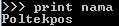
\includegraphics[width=0.55\textwidth]{figures/2/hasilperintahprint}}
	\caption{Hasil Perintah Print}
	\label{fig:hasilperintahprint}
\end{figure}

\subsection{Menghapus Variabel}
Untuk menghapus variabel caranya sangat mudah. Anda cukup menggunakan perintah del() untuk menghapus variabel yang sudah tidak dibutuhkan lagi. Perintah delete, \verb|del(namavariabel)|
Contohnya seperti pada gambar \ref{fig:perintahdel} :
\begin{figure}[!htbp]
	\centerline{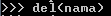
\includegraphics[width=0.40\textwidth]{figures/2/perintahdel.PNG}}
	\caption{Perintah del}
	\label{fig:perintahdel}
\end{figure}

Untuk mengecek apakah variabelnya berhasil dihapus anda bisa menggunakan perintah print seperti pada gambar \ref{fig:perintahprint}. 
\begin{figure}[!htbp]
	\centerline{
\includegraphics[width=0.55\textwidth]{figures/2/perintahprint.PNG}}
	\caption{Perintah Print}
	\label{fig:perintahprint}
\end{figure}

Jika hasilnya seperti gambar \ref{fig:afterdelete} maka variabel telah berhasil dihapus.
\begin{figure}[!htbp]
	\centerline{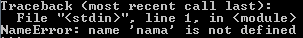
\includegraphics[width=0.75\textwidth]{figures/2/afterdelete.PNG}}
	\caption{Hasil perintah print setelah variabel di delete}
	\label{fig:afterdelete}
\end{figure}

\section{Input Output User}
Input adalah masukan yang anda berikan kepada sebuah program dan system akan memproses lalu menampilkan ouputnya.

\subsection{Cara mengambil input pada keyboard}
Di dalam python sudah terdapat fungsi input() dan raw\_input(). input() digunakan untuk masukan bernilai angka sedangkan raw\_input untuk masukan bernilai teks.

Cara penggunaannya seperti ini \verb|nama\_variabel = input(“masukkan teks”)|

Teks yang anda masukkan akan disimpan ke nama\_variabel.

Contohnya seperti pada listing \ref{lst:iouser} :
\lstinputlisting[caption=Contoh kode input output, label={lst:iouser}]{src/2/iouser.py}

Hasilnya seperti pada gambar \ref{fig:hasilinput}:
\begin{figure}[!htbp]
	\centerline{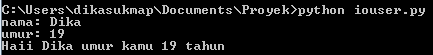
\includegraphics[width=0.85\textwidth]{figures/2/hasilinput.PNG}}
	\caption{Hasil input}
	\label{fig:hasilinput}
\end{figure}

\subsection{Menampilkan Variabel dan Teks}
Anda bisa menampilkan variabel dan teks menggunakan perintah print seperti pada listing \ref{lst:halo}
\lstinputlisting[caption=Perintah menampilkan variabel dan teks, label={lst:halo}]{src/2/halo.py}

Hasilnya seperti pada gambar \ref{fig:showvar}:
\begin{figure}[!htbp]
	\centerline{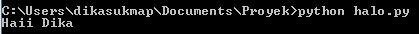
\includegraphics[width=0.85\textwidth]{figures/2/showvar.PNG}}
	\caption{Hasil menampilkan variabel dan teks}
	\label{fig:showvar}
\end{figure}

Tanda koma pada kode diatas merupakan sebuah spasi apabila kode dieksekusi.

\section{Operator Dasar}
Operator python adalah simbol yang melakukan operasi pada satu atau lebih operan. Operan adalah variabel atau nilai yang digunakan untuk melakukan operasi.
Operator pada Python dibagi menjadi beberapa jenis, yaitu :

\subsection{Operator Aritmatika}
% Please add the following required packages to your document preamble:
% \usepackage{graphicx}
\begin{table}[]
\caption{Operator Aritmatika}
\label{tab:my-table}
\resizebox{\textwidth}{!}{%
\begin{tabular}{|l|l|l|}
\hline
Operator           & Contoh      & Keterangan                                                                                                 \\ \hline
Penjumlahan +      & 3 + 1 = 4   & Menjumlahkan masing - masing bilangan                                                                      \\ \hline
Pengurangan -      & 4 - 1 = 3   & Mengurangi nilai operan di sebelah kiri menggunakan operan di sebelah kanan                                \\ \hline
Perkalian *        & 2 * 1 = 2   & Mengalikan dua bilangan                                                                                    \\ \hline
Pembagian /        & 4 / 2 = 2   & Untuk membagi operan di sebelah kiri menggunakan operan di sebelah kanan                                   \\ \hline
Sisa Bagi \%       & 13 \% 4 = 1 & Mendapatkan sisa pembagian dari operan di sebelah kiri operator ketika dibagi oleh operan di sebelah kanan \\ \hline
Pangkat **         & 6 ** 2 = 36 & Memangkatkan operan disebelah kiri operator dengan operan di sebelah kanan operator                        \\ \hline
Pembagian Bulat // & 10 // 3 = 3 & Sama seperti pembagian. Hanya saja angka dibelakang koma dihilangkan                                       \\ \hline
\end{tabular}%
}
\end{table}

Contoh penggunaannya seperti pada listing \ref{lst:aritmatika} :
\lstinputlisting[caption=Contoh operator aritmatika, label={lst:aritmatika}]{src/2/operator_aritmatika.py}

Hasilnya seperti pada gambar \ref{fig:aritmatika}:
\begin{figure}[!htbp]
	\centerline{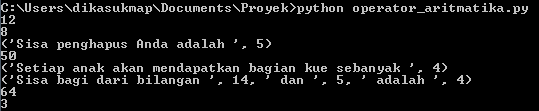
\includegraphics[width=0.85\textwidth]{figures/2/aritmatika.PNG}}
	\caption{Hasil contoh operator aritmatika}
	\label{fig:aritmatika}
\end{figure}

\subsection{Operator Perbandingan}
% Please add the following required packages to your document preamble:
% \usepackage{graphicx}
\begin{table}[]
\caption{Operator Perbandingan}
\label{tab:my-table}
\resizebox{\textwidth}{!}{%
\begin{tabular}{lll}
Operator                                    & Contoh                      & Keterangan                                                                                                       \\
Sama dengan =                               & 2 == 2                      & bernilai True Jika masing-masing operan memiliki nilai yang sama, maka kondisi bernilai benar atau True.         \\
Tidak sama dengan !=                        & 2 != 2                      & bernilai False Akan menghasilkan nilai kebalikan dari kondisi sebenarnya.                                        \\
Tidak sama dengan \textless{}\textgreater{} & 2 \textless{}\textgreater 2 & bernilai False Akan menghasilkan nilai kebalikan dari kondisi sebenarnya                                         \\
Lebih besar dari \textgreater{}             & 3 \textgreater 2            & bernilai True Jika nilai operan kiri lebih besar dari nilai operan kanan, maka kondisi menjadi benar.            \\
Lebih kecil dari \textless{}                & 2 \textless 3               & bernilai True Jika nilai operan kiri lebih kecil dari nilai operan kanan, maka kondisi menjadi benar.            \\
Lebih besar / sama dengan \textgreater{}=   & 3 \textgreater{}= 2         & bernilai True Jika nilai operan kiri lebih besar dari nilai operan kanan, atau sama, maka kondisi menjadi benar. \\
Lebih kecil / sama dengan =                 & 2 \textless{}= 3            & bernilai True Jika nilai operan kiri lebih kecil dari nilai operan kanan, atau sama, maka kondisi menjadi benar.
\end{tabular}%
}
\end{table}

Contoh penggunaannya seperti pada listing \ref{lst:perbandingan} :
\lstinputlisting[caption=Contoh operator perbandingan, label={lst:perbandingan}]{src/2/operator_perbandingan.py}

Hasilnya seperti pada gambar \ref{fig:perbandingan}:
\begin{figure}[!htbp]
	\centerline{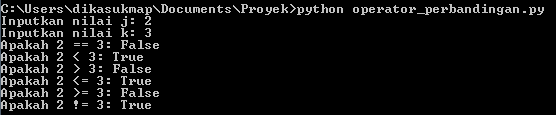
\includegraphics[width=0.85\textwidth]{figures/2/perbandingan.PNG}}
	\caption{Hasil contoh operator perbandingan}
	\label{fig:perbandingan}
\end{figure}

\subsection{Operator Penugasan}
Operator Penugasan digunakan untuk memodifikasi sebuah nilai yang ada pada variabel tertentu.
% Please add the following required packages to your document preamble:
% \usepackage{graphicx}
\begin{table}[]
\caption{Operator Penugasan}
\label{tab:my-table}
\resizebox{\textwidth}{!}{%
\begin{tabular}{lll}
Operator                        & Contoh  & Penjelasan                                                                                                                                   \\
Sama dengan =                   & A = 3   & Memberikan nilai di kanan ke dalam variabel yang berada di sebelah kiri.                                                                     \\
Tambah sama dengan +=           & A += 3  & Memberikan nilai variabel dengan nilai variabel itu sendiri ditambah dengan nilai di sebelah kanan.                                          \\
Kurang sama dengan -=           & A -= 3  & Memberikan nilai variabel dengan nilai variabel itu sendiri dikurangi dengan nilai di sebelah kanan.                                         \\
Kali sama dengan *=             & A *= 3  & Memberikan nilai variabel dengan nilai variabel itu sendiri dikali dengan nilai di sebelah kanan.                                            \\
Bagi sama dengan /=             & A /= 6  & Memberikan nilai variabel dengan nilai variabel itu sendiri dibagi dengan nilai di sebelah kanan.                                            \\
Sisa bagi sama dengan  \%=      & A \%= 3 & Memberikan nilai variabel dengan nilai variabel itu sendiri dibagi dengan nilai di sebelah kanan. Yang diambil nantinya adalah sisa baginya. \\
Pangkat sama dengan **=         & A **= 2 & Memberikan nilai variabel dengan nilai variabel itu sendiri dipangkatkan dengan nilai di sebelah kanan.                                      \\
Pembagian bulat sama dengan //= & A //= 4 & Membagi bulat operan sebelah kiri operator dengan operan sebelah kanan operator kemudian hasilnya diisikan ke operan sebelah kiri.          
\end{tabular}%
}
\end{table}

Contoh penggunaannya seperti pada listing \ref{lst:penugasan} :
\lstinputlisting[caption=Contoh operator penugasan, label={lst:penugasan}]{src/2/operator_penugasan.py}

Hasilnya seperti pada gambar \ref{fig:penugasan}:
\begin{figure}[!htbp]
	\centerline{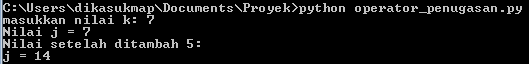
\includegraphics[width=0.85\textwidth]{figures/2/penugasan.PNG}}
	\caption{Hasil contoh operator penugasan}
	\label{fig:penugasan}
\end{figure}

\subsection{Operator Logika}
Operator logika digunakan untuk membuat operasi logika, seperti logika AND, OR, dan NOT.

\begin{table}[]
\caption{Operator Logika}
\label{tab:my-table}
\begin{tabular}{|l|l|}
\hline
Nama             & Simbol \\ \hline
Logika And       & and    \\ \hline
Logika Or        & or     \\ \hline
Negasi/kebalikan & not    \\ \hline
\end{tabular}
\end{table}

Contoh penggunaannya seperti pada listing \ref{lst:logika} :
\lstinputlisting[caption=Contoh operator logika, label={lst:logika}]{src/2/operator_logika.py}

Hasilnya seperti pada gambar \ref{fig:logika}:
\begin{figure}[!htbp]
	\centerline{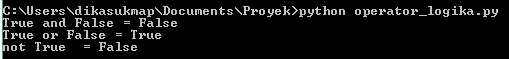
\includegraphics[width=0.85\textwidth]{figures/2/logika.PNG}}
	\caption{Hasil contoh operator logika}
	\label{fig:logika}
\end{figure}

\subsection{Operator Bitwise}
Operator bitwise digunakan untuk melakukan operasi dalam bentuk bit atau biner.

\begin{table}[]
\caption{Operator Bitwise}
\label{tab:my-table}
\begin{tabular}{|l|l|}
\hline
Nama        & Simbol                       \\ \hline
AND         & \&                           \\ \hline
OR          & |                            \\ \hline
XOR         & \textasciicircum{}           \\ \hline
Negasi      & $\sim$                       \\ \hline
Left Shift  & \textless{}\textless{}       \\ \hline
Right Shift & \textgreater{}\textgreater{} \\ \hline
\end{tabular}
\end{table}

Contoh penggunaannya seperti pada listing \ref{lst:bitwise} :
\lstinputlisting[caption=Contoh operator bitwise, label={lst:bitwise}]{src/2/operator_bitwise.py}

Hasilnya seperti pada gambar \ref{fig:bitwise}:
\begin{figure}[!htbp]
	\centerline{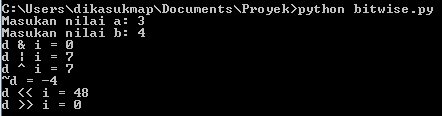
\includegraphics[width=0.85\textwidth]{figures/2/bitwise.PNG}}
	\caption{Hasil contoh operator bitwise}
	\label{fig:bitwise}
\end{figure}

\subsection{Prioritas Eksekusi Operator di Python}
Berikut adalah prioritas yang dieksekusi di dalam perintah python. Maksudnya adalah di dalam python terdapat beberapa operator dan prioritasnya masing - masing. Tabel \ref{tab:eksekusi} merupakan prioritas python dari mulai yang pertama sampai dengan yang terakhir dalam proses pengeksekusian :
\begin{table}[]
\caption{Prioritas Eksekusi Operator di Python}
\label{tab:my-table}
\begin{tabular}{|l|l|}
\hline
Operator                                                & Keterangan   \\ \hline
**                                                      & Aritmatika   \\ \hline
$\sim$,+,-                                              & Bitwise      \\ \hline
*,/,//,\%                                               & Arimatika    \\ \hline
+,-                                                     & Aritmatika   \\ \hline
\textgreater{}\textgreater{},\textless{}\textless{}     & Bitwise      \\ \hline
\&                                                      & Bitwise      \\ \hline
\textasciicircum{},|                                    & Bitwise      \\ \hline
\textless{}=,\textless{},\textgreater{},\textgreater{}= & Perbandingan \\ \hline
\textless{}\textgreater{},==,!=                         & Perbandingan \\ \hline
Err:509                                                 & Penugasan    \\ \hline
Is,is not                                               & Identitas    \\ \hline
In,not in                                               & Keanggotaan  \\ \hline
Not,or,and                                              & Logika       \\ \hline
\end{tabular}
\end{table}

\section{Perulangan / Loop}
Secara umum, perintah pada bahasa pemrograman Python akan dijalankan secara berurutan. Pernyataan pertama dalam sebuah fungsi dijalankan pertama, lalu diikuti oleh yang kedua, dan seterusnya. Tetapi akan ada situasi dimana Anda harus menulis banyak kode, dimana kode tersebut sangat banyak. Jika dilakukan secara manual maka Anda hanya akan membuang-buang waktu dan tenaga. Untuk itu Anda perlu menggunakan pengulangan atau loop di dalam bahasa pemrograman Python.

Di dalam bahasa pemrograman Python pengulangan dibagi menjadi 3 bagian, yaitu :
\subsection{While Loop}
Pada while loop pernyataan akan dieksekusi berkali-kali selama kondisi bernilai benar atau true.

Contoh penggunaannya seperti pada listing \ref{lst:whileloop} :
\lstinputlisting[caption=Koding while loop, label={lst:whileloop}]{src/2/whileloop.py}

\subsection{For Loop}
For Loop memiliki kemampuan untuk mengulangi item dari urutan apapun,misalnya string atau list.

Contoh penggunaannya seperti pada listing \ref{lst:forloop} :
\lstinputlisting[caption=Koding for loop, label={lst:forloop}]{src/2/forloop.py}
 
\subsection{Nested Loop} 
Nested loop memungkinkan terjadi sebuah pengulangan di dalam pengulangan lainnya.

Contoh penggunaannya seperti pada listing \ref{lst:nestedloop} :
\lstinputlisting[caption=Koding nested loop, label={lst:nestedloop}]{src/2/nestedloop.py}

\section{Kondisi}
\subsection{Kondisi IF}
Pada saat pengambilan keputusan (kondisi if) digunakan untuk mengantisipasi kondisi yang akan terjadi saat program dijalankan.Dan akan menentukan tindakan apa yang akan diambil sesuai dengan kondisi program pada saat dieksekusi.

Pada python ada beberapa kondisi diantaranya adalah if, else, dan elif. Kondisi if hanya bisa digunakan pada saat kondisi benar saja.

Contoh penggunaannya seperti pada listing \ref{lst:kondisiif} :
\lstinputlisting[caption=Koding kondisi if, label={lst:kondisiif}]{src/2/kondisiif.py}

Dari contoh tersebut, jika if petama dijalankan maka akan menampilkan “Selamat Ulang Tahun” sebanyak 1 kali, di statement ke 2 perintah print("Selamat Ulang Tahun") tidak akan dieksekusi karena statement bernilai salah.

\subsection{Kondisi IF Else}
Pengambilan kondisi IF Else tidak hanya mengeksekusi jika program yang telah ditetapkan bernilai benar, tetapi kondisi IF Else juga menentukan tindakan apa yang diambil jika sebuah program bernilai salah atau tidak sesuai.
Di dalam kondisi IF Else, perintah IF akan dijalankan jika pernyataan yang dieksekusi benar. Sedangkan jika pernyataan yang dieksekusi salah maka yang akan dijalankan adalah perintah Else.

Contoh penggunaannya seperti pada listing \ref{lst:kondisiifelse} :
\lstinputlisting[caption=Koding kondisi if else, label={lst:kondisiifelse}]{src/2/kondisiifelse.py}

Pada program diatas pernyataan bernilai salah, maka yang akan dieksekusi adalah perintah else dan akan menampilkan “Maaf anda tidak ulang tahun hari ini”.

\subsection{Kondisi Elif}
Kondisi if elif merupakan percabangan logikan dari “kondisi if”. Dengan Elif anda bisa membuat kondisi program menjadi banyak pilihan. Dan kondisi ini akan menyeleksi kemungkinan yang akan terjadi. Kondisi ini memiliki banyak pilihan, ini merupakan perbedaan dari kondisi elif dan kondisi if else.

Contoh penggunaannya seperti pada listing \ref{lst:kondisielif} :
\lstinputlisting[caption=Koding kondisi elif, label={lst:kondisielif}]{src/2/kondisielif.py}

Karena pernyataan diatas adalah hari minggu maka akan dieksekusi pada saat hari minggu dan akan menampilkan “ Saya akan libur”.

\section{Pembacaan Error}
Pada saat membuat suatu program, terkadang program tidak berjalan seperti yang  diinginkan. Anda harus mengetahui error apa yang terjadi dengan program yang telah dibuat. Berikut adalah 2 macam error yang terjadi pada python.
\subsection{Kesalahan sintak} 
Biasanya yang paling mudah dikenali, kesalahan sintaksis terjadi ketika Anda membuat kesalahan ketik. Tidak mengakhiri pernyataan if dengan titik dua adalah contoh kesalahan sintak, seperti salah mengeja kata kunci Python (mis. Menggunakan whille alih-alih sementara). Kesalahan sintak biasanya muncul pada waktu kompilasi dan dilaporkan oleh interpreter. 
Contoh penggunaannya seperti pada listing \ref{lst:error} :
\lstinputlisting[caption=Koding kesalahan sintak, label={lst:error}]{src/2/error.py}

Hasilnya seperti pada gambar \ref{fig:error}:
\begin{figure}[!htbp]
	\centerline{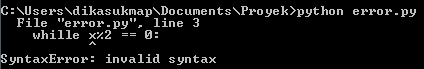
\includegraphics[width=0.85\textwidth]{figures/2/error.PNG}}
	\caption{Hasil menangkap pengecualian khusus}
	\label{fig:error}
\end{figure}
Kesalahan terdapat pada “whille”, perintah tersebut harusnya tidak menggunakan doubel l tetapi “while”.

\subsection{Kesalahan Logika}
Juga disebut kesalahan semantik, kesalahan logis menyebabkan program berperilaku tidak benar, tetapi mereka biasanya tidak crash program. Tidak seperti program dengan kesalahan sintaks, program dengan kesalahan logika dapat dijalankan, tetapi tidak beroperasi sebagaimana dimaksud. 

Pertimbangkan contoh kesalahan logis seperti pada listing \ref{lst:kesalahanlogika}:
\lstinputlisting[caption=Koding kesalahan logika, label={lst:kesalahanlogika}]{src/2/kesalahanlogika.py}

Contoh di atas harus menghitung rata-rata dari dua angka yang dimasukkan pengguna. Tetapi, karena urutan operasi dalam aritmatika (pembagian dievaluasi sebelum penambahan) program tidak akan memberikan jawaban yang benar seperti pada gambar \ref{fig:salahlogika}:
\begin{figure}[!htbp]
	\centerline{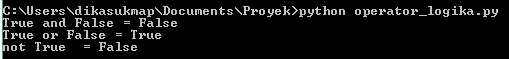
\includegraphics[width=0.85\textwidth]{figures/2/salahlogika.PNG}}
	\caption{Hasil program kesalahan logika}
	\label{fig:salahlogika}
\end{figure}

Untuk memperbaiki masalah ini, cukup menambahkan tanda kurung: z = (x + y) / 2
Ini adalah hasil yang benar seperti pada gambar \ref{fig:benarlogika}:
\begin{figure}[!htbp]
	\centerline{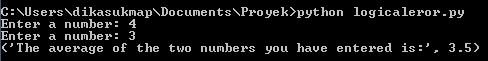
\includegraphics[width=0.85\textwidth]{figures/2/benarlogika.PNG}}
	\caption{Hasil setelah di benarkan}
	\label{fig:benarlogika}
\end{figure}

\section{Try to Except/pengecualian}
Python memiliki banyak exceptions bawaan yang memaksa program Anda untuk menghasilkan kesalahan ketika ada sesuatu yang salah di dalamnya. Ketika exceptions ini terjadi, itu menyebabkan proses saat ini berhenti dan meneruskannya ke proses panggilan sampai ditangani. Jika tidak ditangani, program ini akan macet.

Misalnya, jika fungsi A memanggil fungsi B yang pada gilirannya memanggil fungsi C dan pengecualian terjadi di fungsi C. Jika tidak ditangani dalam C, pengecualian beralih ke B dan kemudian ke A. Jika tidak pernah ditangani, pesan kesalahan dilemparkan dan program ini terhenti secara tiba-tiba.

\subsection{Menangkap Pengecualian dengan Python}
Dalam Python, pengecualian dapat ditangani menggunakan pernyataan coba. Operasi kritis yang dapat meningkatkan pengecualian ditempatkan di dalam klausa coba dan kode yang menangani pengecualian ditulis dalam kecuali klausa.

Contoh penggunaannya seperti pada listing \ref{lst:exception} :
\lstinputlisting[caption=Koding exception, label={lst:exception}]{src/2/exception.py}

Hasilnya seperti pada gambar \ref{fig:exception}:
\begin{figure}[!htbp]
	\centerline{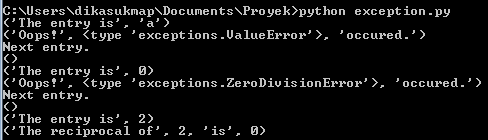
\includegraphics[width=0.85\textwidth]{figures/2/exception.PNG}}
	\caption{Hasil try to except}
	\label{fig:exception}
\end{figure}

Dalam program ini, anda harusi mengulang sampai pengguna memasukkan bilangan bulat yang memiliki timbal balik yang valid. Bagian yang dapat menyebabkan pengecualian ditempatkan di dalam blok try.

Jika tidak ada pengecualian terjadi, kecuali blok dilewati dan aliran normal berlanjut. Tetapi jika ada pengecualian terjadi, itu ditangkap oleh blok kecuali. System mencetak nama pengecualian menggunakan fungsi ex\_info () di dalam modul sys dan meminta pengguna untuk mencoba lagi. Anda dapat melihat bahwa nilai 'a' dan '1,3' menyebabkan ValueError dan '0' menyebabkan ZeroDivisionError.

\subsection{Menangkap Pengecualian Khusus dengan Python}
Dalam contoh di atas, pengecualian dalam klausa kecuali tidak disebutkan. Ini bukan praktik pemrograman yang baik karena akan menangkap semua pengecualian dan menangani setiap kasus dengan cara yang sama. Anda dapat menentukan pengecualian mana yang dikecualikan klausa kecuali.

Klausa coba dapat memiliki sejumlah kecuali klausa untuk menanganinya secara berbeda tetapi hanya satu yang akan dieksekusi jika terjadi pengecualian. Anda bisa menggunakan tupel nilai untuk menentukan beberapa pengecualian dalam klausa kecuali. 

Contoh penggunaannya seperti pada listing \ref{lst:specialexception} :
\lstinputlisting[caption=Koding special exception, label={lst:specialexception}]{src/2/specialexception.py}

\subsection{Meningkatkan Pengecualian}
Dalam pemrograman Python, pengecualian dimunculkan ketika kesalahan yang sesuai terjadi pada waktu berjalan, tetapi dapat dengan paksa menaikkannya menggunakan peningkatan kata kunci. Anda juga bisa memberikan nilai secara opsional pada pengecualian untuk mengklarifikasi mengapa pengecualian itu dinaikkan.

Contoh penggunaannya seperti pada listing \ref{lst:upexception} :
\lstinputlisting[caption=Koding meningkatkan pengecualian, label={lst:upexception}]{src/2/upexception.py}

\subsection{Try Finally}
Pernyataan coba dengan Python dapat memiliki klausa finally opsional. Klausa ini dieksekusi apa pun yang terjadi, dan umumnya digunakan untuk melepaskan sumber daya eksternal. Misalnya, anda dapat terhubung ke pusat data jarak jauh melalui jaringan atau bekerja dengan file atau bekerja dengan Graphical User Interface (GUI). 

Dalam semua keadaan ini, anda harus membersihkan sumber daya yang pernah digunakan, apakah itu berhasil atau tidak. Tindakan-tindakan ini (menutup file, GUI atau memutuskan sambungan dari jaringan) dilakukan pada klausa terakhir untuk menjamin eksekusi.

Contoh penggunaannya seperti pada listing \ref{lst:tryfinnaly} :
\lstinputlisting[caption=Koding try finnaly, label={lst:tryfinnaly}]{src/2/tryfinnaly.py}

Tipe konstruksi ini memastikan file ditutup bahkan jika pengecualian terjadi.

\chapter{Pengenalan Flask}
\section{Definisi \textit{Micro Frameworki}}

\textit{Microframework} adalah istilah yang digunakan untuk merujuk pada kerangka kerja web minimalis. Kerangka ini sangat berbeda dengan kerangka kerja tumpukan penuh. Juga tidak memiliki sebagaian besar fungsionalitas yang umum yang ada dalam kerangka kerja aplikasi web lengkap, seperti:
\begin{enumerate}
\item Akun, otentikasi, otorisasi, peran, dll.
\item Abtraksi basis data melalui pemetaan objek-relasional.
\item Validai  \textit{input} dan sanitasi \textit{input}.
\item Mesin \textit{template web}.
\end{enumerate}

Biasanya, sebuah \textit{microframework} memfasilitasi menerima permintaan HTTP, merutekan permintaan HTTP ke \textit{controller} yang sesuai, mengirim \textit{controller}, dan mengembalikan respons HTTP. \textit{Microframeworks} seringkali dirancang khusus untuk membangun API untuk layanan atau aplikasi lain. Misalnya, Lumen \textit{microframework} dirancang untuk pengembangan \textit{Microservices} dan pengembangan API. \textit{Microframework}, sebuah \textit{tool} yang digunakan untuk \textit{project} yang lebih kecil dan penggunaan untuk kasus yang spesifik. Ini sama saja dengan menyederhanakan \textit{framework} agar lebih mudah dalam implementasi dan menyediakan \textit{testing} dan \textit{deployment} yang lebih cepat. \textit{Microframework} mengeluarkan banyak sekali komponen yang ada pada pengaturanan \textit{full-stack}, termasuk:
\begin{enumerate}
\item \textit{Web template engine}
\item \textit{Input validation}
\item \textit{Database abstraction}
\item \textit{Roles, accounts, and authentication}
\end{enumerate}

Kerugian menggunakan  \textit{microframework} adalah saat  \textit{project} mulai tumbuh besar dengan cepat. Dimana  \textit{microframework} tidak memiliki fitur yang dibutuhkan untuk mengakomodasi pertumbuhan  \textit{website}. Dengan kata lain kamu kehilangan fleksibelitas.  \textit{Micro-framework} lebih baik saat digunakan untuk  \textit{project} kecil yang membutuhkan kesederhanaan,  \textit{overhead} yang rendah dan  \textit{deployment} yang cepat.  \textit{Developer} yang sudah berpengalaman bisa saja menggunakan  \textit{microframework} pada awal  \textit{project} dan menambahkan tambahan  \textit{microframework} jika diperlukan. Hal ini merupakan pilihan yang menarik, tetapi untuk pemula dan  \textit{developer} menengah harus menghindari ini \cite{fadhilnet}.

\section{Jenis-Jenis \textit{Framework} Python serta Kelebihan dan Kekurangan}

\subsection{Django}

Django adalah kerangka kerja web Python yang memungkinkan individu dalam pengembangan yang bersih dan cepat. Kerangka kerja web secara umum dikatakan sebagai campuran komponen yang membantu pengembang mengembangkan situs web lebih cepat dan mudah. Karena itu, ini adalah kerangka kerja sumber bebas dan terbuka. Ini dapat disebut sebagai kerangka kerja yang memungkinkan pengembang untuk mengambil konsep penyelesaian secepat mungkin. Django sebagai kerangka kerja membantu mengurangi beberapa kesalahan keamanan umum yang dapat diawasi dengan mudah saat mengembangkan aplikasi. Skalabilitas adalah fitur lain yang disediakan oleh kerangka ini.

Django memiliki \textit{tagline "The web framework for perfectionists with deadlines"}, bagaimana tidak, karena secara \textit{default} Django sudah memiliki berbagai modul umum yang biasa digunakan ketika mengembangkan aplikasi web.

Kelebihan:
\begin{enumerate}
\item Cepat.

Ini telah dirancang sedemikian rupa untuk membantu pengembang membuat aplikasi secepat mungkin. Dari ide, produksi hingga rilis, Django membantu menjadikannya efektif dan efisien. Dengan demikian itu menjadi solusi ideal bagi pengembang yang memiliki fokus utama pada tenggat waktu.

\item Penuh dimuat.

Ini bekerja dengan cara yang mencakup puluhan tambahan untuk membantu dengan otentikasi pengguna, peta situs, administrasi konten, umpan RSS, dan banyak lagi hal-hal seperti itu. Aspek-aspek ini membantu dalam melaksanakan proses pengembangan web sepenuhnya.

\item Aman.

Ketika melakukannya di Django, dipastikan bahwa pengembang tidak melakukan kesalahan yang terkait dengan keamanan. Beberapa kesalahan umum termasuk injeksi SQL, pemalsuan permintaan lintas situs, clickjacking dan skrip lintas situs. Untuk mengelola nama pengguna dan kata sandi secara efektif, sistem otentikasi pengguna adalah kuncinya.

\item Dapat diukur.

Untuk memenuhi permintaan lalu lintas terberat, manfaat kerangka Django dapat dilihat. Oleh karena itu, situs tersibuk menggunakan media ini untuk dengan cepat memenuhi permintaan lalu lintas.

\item Serbaguna.

Manajemen konten,\textit{ platform} komputasi ilmiah, dan bahkan organisasi besar, semua aspek ini dikelola secara efisien dengan penggunaan Django.

\item Dokumentasi yang sangat lengkap dan kamu tidak perlu banyak - banyak \textit{googling} karena sudah disediakan contoh.
\item Modul administrasi yang \textit{auto generate} sesuai dengan model yang didefinisikan di dalam aplikasi. Lebih dari sekedar \textit{CRUD generator}.
\item Sistem migrasi \textit{database} otomatis yang tidak perlu kamu tulis \textit{script}-nya. Cukup mengubah class dan struktur \textit{database} pun berubah sesuai perubahan terakhir.
\item Memiliki sistem form yang kokoh.
\item Sudah \textit{built-in} untuk sistem autentikasi dan roles bila Anda menggunakan \textit{relational database} yang didukung Django seperti MySQL dan PostgreSQL.
\item Memiliki ekstensi - ekstensi yang bisa membuat kamu lebih produktif seperti \textit{Django Rest Framework, Django Rest Auth, Django Celery, Django Mongoengine, GeoDjango,} dan lainnya.
\item Memiliki \textit{template engine} sendiri yang lebih \textit{powerful}.
\item Kompatibilitas dengan berbagai modul dan \textit{library} lain.
\end{enumerate}

Kekurangan:
\begin{enumerate}
\item Menggunakan pola perutean, tentukan URL-nya
\item Django terlalu monolitik
\item Semuanya didasarkan pada Django ORM
\item Komponen dikerahkan bersama
\item Pengetahuan tentang sistem lengkap diperlukan untuk bekerja.
\end{enumerate}

\subsection{Flask}

Python adalah Flask, yang merupakan kerangka kerja mikro untuk Python berdasarkan teknologi seperti Werkzeug, Jinja 2. Flask pada dasarnya adalah kerangka kerja web Python yang dibangun dengan inti kecil dan selanjutnya mudah untuk memperpanjang ekstensi Flask lebih berorientasi Python daripada Django karena beberapa alasan yang jelas. Karena ada sedikit kode \textit{boilerplate} yang harus ditangani oleh pengembang, Flask adalah kerangka kerja web yang mungkin tidak perlu dikerjakan pengembang lebih lama untuk memahami mereka. Banyak aplikasi terkenal di luar sana ditulis dalam kerangka kerja Flask seperti Pinterest, LinkedIn dan halaman web komunitas untuk Flask itu sendiri \cite{ramdani2018clustering}.

Flask sendiri dapat dikatakan sebagai \textit{web framework} yang fleksibel terhadap library apapun untuk Python. Selain itu dokumentasinya yang jelas membuat Flask sangat diminati oleh kawula muda.

Kelebihan:

\begin{itemize}
	\item \textit{Framework} yang mudah untuk digunakan dan dipahami.
	\item Berisi pengembangan server dan \textit{debugger}.
	\item \textit{RESTfull request dispatching}.
	\item Menggunakan Jinja2 \textit{template engine}.
	\item Dukungan untuk \textit{secure cookies} pada sisi \textit{client}.
	\item 100\% \textit{Web Server Gateway Interface} (WSGI).
	\item Berbasis \textit{Unicode} yaitu suatu standar yang dirancang untuk mengizinkan \textit{text} dan \textit{symbol} dari semua tulisan untuk menampilkan dan dimanipulasi secara konsisten oleh komputer.
	\item Dokumentasi yang ekstensif.
	\item Kompatibilitas \textit{Google App Engine}.
\end{itemize}

Kekurangan:
\begin{itemize}
\item Fungsionalitas
\end{itemize}

Beberapa fitur Flask yang perlu kamu ketahui antara lain:
\begin{itemize}
	\item \textit{Built-in development server} dan \textit{debugger}.
	\item Terintegrasi dengan unit \textit{testing}.
	\item RESTful.
	\item Menggunakan \textit{template engine} Jinja2.
	\item Mendukung \textit{secure cookie}.
	\item 100\% mendukung WSGI 1.0.
	\item \textit{Unicode based}.
	\item Dokumentasi yang baik.
	\item Komunitas yang kuat.
\end{itemize}

\section{Instalasi dan Hello World di Flask}

\subsection{Instalasi Python 2.7.}

Mulai dengan tutorial dalam menginstall Python 2.7. Python ini digunakan untuk \textit{code} pembaca data dari sinyal gelombang otak yang telah dihasilkan oleh alat EEG yaitu NeuroSky Mindwave. Baiklah langsung kita mulai saja:
\begin{enumerate}
\item Pertama-tama silahkan download software dari python versi 2 di laptop anda. Download python versi 2.7.15 dari situs web resminya yaitu https://www.python.org/. Silahkan sesuaikan dengan kapasitas laptop anda, bisa yang win 32 atau yang win 64 (32 bit / 64 bit). Contoh downloadnya seperti pada gambar \ref{fig:python}.
\begin{figure}[!htbp]
	\centerline{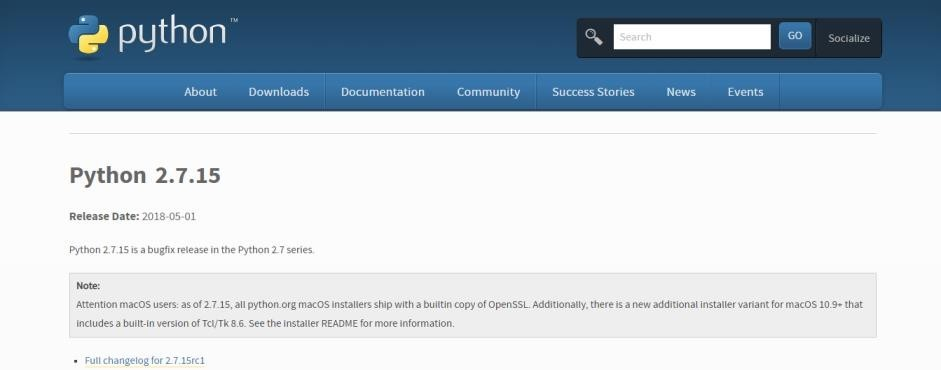
\includegraphics[width=1\textwidth]{figures/8/python.jpg}}
	\caption{Download Softfile Python 2.7.}
	\label{fig:python}
\end{figure}

\item Setelah di \textit{download}  silahkan  buka  Command  Prompt  di komputer/PC anda.
\item Kemudian silahkan ketikkan perintah \verb|pip install flask|.
\item Setelah mengetikkan perintah tersebut, silahkan tekan \textit{enter} maka prosesnya akan berjalan. Silahkan tunggu hasilnya. Hasilnya akan nampak seperti gambar \ref{fig:cek_python}.
\begin{figure}[!htbp]
	\centerline{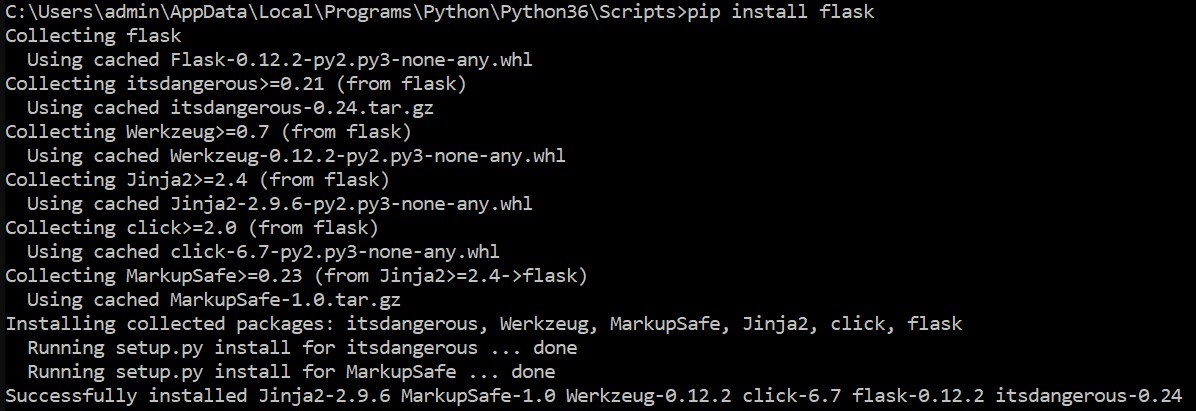
\includegraphics[width=1\textwidth]{figures/8/cek_python.jpg}}
	\caption{Froses Instalasi Flask}
	\label{fig:cek_python}
\end{figure}

\end{enumerate}

Perintah python flask. Contoh \textit{source code} seperti pada listing \ref{lst:hello}.
\lstinputlisting[caption=Contoh kode program hello.py, label={lst:hello}]{src/8/hello.py}
 Contoh \textit{source code} main.py seperti pada listing \ref{lst:main}.
\lstinputlisting[caption=Contoh kode program main.py, label={lst:main}]{src/8/main.py}


\chapter{HTTP GET METHOD REQUEST}
\section{HTTP Method Request}
\subsection{Pengertian HTTP Method Request}
Protokol HTTP adalah protokol permintaan atau respon. Klien mengirimkan permintaan keserver dalam bentuk metode permintaan, URL, dan versi protokol, diikuti oleh pesan seperti MIME yang berisi perubahan permintaa, informasi klien, dan kemungkinan onten tubuh melalui koneksi dengan server\cite{wyler2005aggressive}. Protokol ini sangat ringan serta generik dan tidak berstatus sehingga dapat dipergunakan oleh tipe dokumen apa saja. Method adalah sekumpulan kode yang diberi namma, untuk merujuk kesekumpulan kode yang ada kemuadian digunakan sebuah nama yang disebut dengan nama method. Method sendiri mempunyai parameter sebagai input (masukan) dan nilai kembalian sebagai output (keluaran). Request adalah permiintaan dimana fungsi ini digunakan sebagai istilah ataupun kinerja dalam pengembalian nilai dari masukan yang dieksekusi.

Berdasarkan beberapa penjelasann diatas, maka untuk pengertian dari HTTP Method Request sendiri merupakan seperangkat metode permintan untuk menunjukkan tindakan yang diinginkan yang akan dilakukan untuk sumber daya tertentu. Meskipun mereka juga bisa menjadi kata benda, metode permintaan ini kadang-kadang disebut sebagai verba HTTP. Masing-masing menerapkan semantik yang berbeda, namun beberapa fitur umum digunakan bersama oleh mereka adalah misalnya Metode pertmintaan dapat berupa safe, idempotent, atau cacheable.

\subsection{Jenis-jenis HTTP Method Request}
\begin{enumerate}
  \item GET : akan dijelaskan pada point berikutnya.
  \item HEAD : Metode HEAD meminta tanggapan yang identik dengan permintaan GET, namun tanpa respon body.
  \item POST : Metode POST digunakan untuk mengirimkan entitas ke sumber daya yang ditentukan, sering menyebabkan perubahan pada keadaan atau efek samping pada server.
  \item PUT : Metode PUT menggantikan semua representasi terkini dari sumber target dengan muatan permintaan.
  \item DELETE : Metode DELETE akan menghapus sumber daya yang ditentukan
  \item CONNECT : Metode CONNECT menetapkan terowongan keserver yang diidentifikasi oleh sumber target.
  \item OPTIONS : Metode OPTIONS digunakan untuk menggambarkan opsi komunikasi untuk sumber target.
  \item TRACE : metode TRACE ini yaitu untuk melakukan tes pesan loop-back disepanjang jalan menuju sumber daya target.
  \item PATCH : Metode PATCH digunakan untuk menerapkan modifikasi sebagian pada sumber daya.
\end{enumerate}

\subsection{Penjelasan Lengkap HTTP Get Method}
Metode GET digunakan untuk meminta representasi suber daya yang ditentukan. permintaan menggunakan Get seharusnya hanya mengambil data. GET adalah salah satu metode HTTP yang paling umum digunakan baik dalam pengimplementasian biasa ataupun sudah dalam bentuk pengujian. Hal yang harus diperhatikan dalam Method Get yaitu :
\begin{itemize}
  \item Permintaan GET dapat di-cache.
  \item Permintaan GET tetap ada dalam riwayat browser.
  \item Permintaan GET dapat ditandai.
  \item Permintaan GET tidak boleh digunakan saat berurusan dengan data sensitif.
  \item Permintaan GET memiliki batasan panjang.
  \item Permintaan GET hanya digunakan untuk meminta data (tidak dimodifikasi).
  \item Permintaan GET dibatasi oleh panjang string sebanyak 2047 karakter.
  \item Permintaan GET memungkinkan pengunjung langsung memasukkan nilai variable pada form proses.
  \item Variabel diambil dengan \$\_REQUEST[“nama”] atau \$\_GET[“nama”]
\end{itemize}

\subsection{Pembacaan HTTP Get Method}
Data dikirimkan dalam HTTP Request dalam dua cara, tergantung dari method yang dikirimkan, yaitu :
\begin{enumerate}
  \item Melalui URL, dengan parameter yang diberikan. Digunakan oleh GET.
  \item Melalui entity body dalam HTTP Request. Digunakan untuk POST dan PUT.
\end{enumerate}

Pada prakteknya terdapat satu cara lagi untuk mengirimkan data, yaitu melalui cookie, tetapi penggunaan cookie tidak akan terlalu efektif karena cookie dirancang untuk menyimpan data status pengguna.

\subsection{Pembacaan Data pada URL}
Pembacaan data yang dikirimkan melalui URL biasanya dilakukan untuk request dengan method GET. Untuk melihat bagaimana GET mengirimkan data, kita terlebih dahulu harus mengerti tentang sintaks penulisan URL. Secara umum, sebuah URL memiliki sintaks seperti berikut :
\lstinputlisting[caption=Contoh kode untuk schema,label={lst:schema}]{src/10/schema.py}
Apa makna dari setiap bagian dari URL yang dijelaskan pada \ref{lst:schema}? Pada tabel \ref{table:schema}, anda dapat melihat makna dan maksud dari contoh URL yang telah diberikan.
\begin{table}[]
\caption{Penjelasan Schema}
\centering
\begin{tabular}{|l|l|l|}
\hline
Nama & Deskripsi & Harus ada ?\\ \hline
schema & Protokol yang digunakan & Ya\\ \hline
user & Nama pengguna & Tidak\\ \hline
password & Password untuk nama pengguna & Tidak\\ \hline
hots & Hostname atau IP & Ya\\ \hline
port & \begin{tabular}[c]{@{}l@{}}Port yang akan diakses. Beberapa atau sebagian\\ protokol memiliki port standar yaitu seperti HTTP = 80\end{tabular} & Tergantung Protokol\\ \hline
paht & Lokasi data pada server & Tergantung Protokol\\ \hline
query & \begin{tabular}[c]{@{}l@{}}Digunakan untuk mengirimkan \\ parameter kepada aplikasi.\end{tabular} & Tidak\\ \hline
fragment & \begin{tabular}[c]{@{}l@{}}Nama dari bagian tertentu pada \\ data (misalnya : judul pada buku)\end{tabular} & Tidak\\ \hline
\end{tabular}
\label{table:schema}
\end{table}

\section {Mekanisme HTTP Method Request}
\subsection{Mekanisme / Alur kerja HTTP Get Method}
Mekanisme adalah suatu rangkaian kerja sebuah alat yang digunakan dalam menyelesaikan sebuah masalah yang berkaitan dengan proses kerja, tujuannya untuk menghasilkan hasil yang mekasimal serta mengurangi datangnya atau munculnya kegagalan. untuk mekanisme HTTP Get Method sendiri dapat diperhatikan sebagai berikut :
\begin{enumerate}
  \item Silahkan membuat dan membangun sebuah URL API.
  \item Didalam URL API (endpoint) tersebut kita akan menggunakan fungsi Method Get.
  \item Kemudian didalam endpoint tersebut akan difungsikan inputan.
  \item Inputan tersebut kemudian akan meghasilkan output (keluaran) dari Metgod GET tersebut.
  \item Secara sederhana, garis besar mekanisme atau alur kerja Method Get nampak seperti penjelasan diatas.
  \item Untuk tutorial pembangunan endpoint seperrti pada point kedua akan dijelaskan pada point selanjutnya.
\end{enumerate}

\section {Contoh URL HTTP Get Method}
Untuk pemberian contoh ini akan dibarengin dengan tutorial pembangunannya, jadi diharapkan teman-teman dapat dengan mudah memahami dan mudah dalam mengikuti contoh yang diberikan. Berikut tutorialnya :
\begin{enumerate}
  \item Endpoint adalah perangkat komputasi jarak jauh yang berkomunikasi bolak-balik dengan jaringan yang terhubung dengannya. Fungsi-fungsi yang dipergunakan yaitu sebagai contoh berikut :
      \begin{itemize}
        \item Fungsi 1 : LoadData.py yaitu membaca file CSV.
            \lstinputlisting[caption=Contoh kode untuk membaca file CSV,label={lst:LoadData}]{src/10/LoadData.py}
        \item Fungsi 2 : Getalldata.py yaitu untuk menampilkan semua data dari file CSV.
            \lstinputlisting[caption=Contoh kode untuk menampilkan semua data dari file CSV,label={lst:GetAllData}]{src/10/GetAllData.py}
        \item Fungsi 3 : Getcolumn.py yaitu untuk menampilkan data dari kolom tertentu.
            \lstinputlisting[caption=Contoh kode untuk menampilkan data dari kolom,label={lst:Getcolumn}]{src/10/Getcolumn.py}
        \item Fungsi 4 : Gettopfive.py yaitu untuk menampilkan 5 data teratas dan terbawah.
            \lstinputlisting[caption=Contoh kode untuk menampilkan 5 data teratas dan terbawah,label={lst:Gettopfive}]{src/10/Gettopfive.py}
        \item Fungsi 5 : Sorting.py yaitu untuk mengurutkan data dari yang terbesar ke yang terkecil dan sebaliknya.
            \lstinputlisting[caption=Contoh kode untuk mengurutkan data,label={lst:Sorting}]{src/10/Sorting.py}
        \item Fungsi 6 : Convertjson.py yaitu untuk mengganti data kedalam format Json.
            \lstinputlisting[caption=Contoh kode untuk mengganti data,label={lst:Convertjson}]{src/10/Convertjson.py}
        \item Fungsi 7 : Deletecolumn.py yaitu untuk menghapus kolom tertentu.
            \lstinputlisting[caption=Contoh kode untuk menghampus kolom tertentu,label={lst:Deletecolumn}]{src/10/Deletecolumn.py}
        \item Fungsi 8 : Deletealldata.py yaitu untuk Menghapus semua data pada file CSV.
            \lstinputlisting[caption=Contoh kode untuk menghapus semua data,label={lst:Deletealldata}]{src/10/Deletealldata.py}
        \item Fungsi 9 : Insertdata.py yaitu untuk menambahkan data.
            \lstinputlisting[caption=Contoh kode untuk menambah data,label={lst:Insertdata}]{src/10/Insertdata.py}
        \item Fungsi 10 : Getinfo.py yaitu untuk Menampilkan data csv namun dengan format json bawaan dari library pandas yang akan berupa deskripsi.
            \lstinputlisting[caption=Contoh kode untuk Menampilkan data csv,label={lst:Getinfo}]{src/10/Getinfo.py}
        \item Fungsi 11 : Getrow.py yaitu untuk Menampilkan seluruh jumlah baris.
            \lstinputlisting[caption=Contoh kode untuk Menampilkan seluruh jumlah baris,label={lst:Getrow}]{src/10/Getrow.py}
        \item Fungsi 12 : Getrowfield.py yaitu untuk Menampilkan data perbaris sesuai dengan kolom yang diiginkan.
            \lstinputlisting[caption=Contoh kode untuk Menampilkan data perbaris,label={lst:Getrowfield}]{src/10/Getrowfield.py}
        \item Fungsi 13 : Updatedata.py yaitu untuk Mengubah data berdasarkan index id.
            \lstinputlisting[caption=Contoh kode untuk Mengubah data berdasarkan index id,label={lst:Updatedata}]{src/10/Updatedata.py}
        \item Fungsi 14 : Deletedata.py yaitu untuk Menghapus data berdasarkan index id.
            \lstinputlisting[caption=Contoh kode untuk Menghapus data berdasarkan index id,label={lst:Deletedata}]{src/10/Deletedata.py}
        \item Fungsi 15 : Getrowjson.py yaitu untuk Mengubah data menjadi Json.
            \lstinputlisting[caption=Contoh kode untuk Mengubah data menjadi Json,label={lst:Getrowjson}]{src/10/Getrowjson.py}
        \item Fungsi 16 : Getalldatajson.py yaitu untuk Menampilkan seluruh data dalam bentuk format Json.
            \lstinputlisting[caption=Contoh kode untuk Menampilkan seluruh data,label={lst:Getalldatajson}]{src/10/Getalldatajson.py}
        \item Fungsi 17 : Amountdata.py yaitu untuk Menghitung jumlah data secara keseluruhan dari kolom dan baris.
            \lstinputlisting[caption=Contoh kode untuk Menghitung jumlah data,label={lst:Amountdata}]{src/10/Amountdata.py}
        \item Fungsi 18 : Getcolumncount.py yaitu untuk Menghitung jumlah kolom pada file.
            \lstinputlisting[caption=Contoh kode untuk Menghitung jumlah kolom,label={lst:Getcolumncount}]{src/10/Getcolumncount.py}
        \item Fungsi 19 : Getrowcount.py yaitu untuk Menghitung jumlah baris pada file.
            \lstinputlisting[caption=Contoh kode untuk Menghitung jumlah baris,label={lst:Getrowcount}]{src/10/Getrowcount.py}
        \item Fungsi 20 : Reloaddata.py yaitu untuk Mengembalikan nilai data.
            \lstinputlisting[caption=Contoh kode untuk Mengembalikan nilai data,label={lst:Reloaddata}]{src/10/Reloaddata.py}
      \end{itemize}

 \subsection{Endpoint 1 (URL API / Dataset)}
  Pembatasan pertama ialah dari Endpoint 1 dimana URL API nya yaitu dataset. Silahkan tuliskan code dibawah sebagai contoh pertama :
  \lstinputlisting[caption=Contoh kode untuk URL API,label={lst:MethodGetfromEndpoint}]{src/10/MethodGetfromEndpoint.py}

  Pada tabel code diatas dapat dilihat bahwa fungsi yang digunakn ialah dataset dimana data set dilakukan pemaggilan fungsi yang ada di file-file yang telah di import. Seperti yang bisa dilihat bahwa pada fungsi dataset direalisasikan dengan metode GET, POST dan DELETE jadi disesuaikan dengan fungsi pada file-file yang dihubungkan atau dipanggil kedalam fungsi dataset. Yang akan dibahas disini adalah MEthod GETnya saja. Tutorialnya sebagai berikut :
  \begin{itemize}
    \item Setelah melakukan perintah \ref{lst:MethodGetfromEndpoint}
    \item Kemudian masukkan perintah yang sesuai
    \item Pendefinisian endpoint dataset
    \item Definisikan request atau permintaan metode yang digunakan. Ada Get 
    \item Pada Method GET : Silahkan masukkan beberapa argument yang akan diolah.
    \item Argumentnya ialah parameter field, topfive, sort dan format
    \item Penjelasan Parameter :
        \subitem All : Mengambil semua data dari file csv
        \subitem Field : Mengambil data berdasarkan parameter field yaitu ada RawValue, sign dan daya
        \subitem Topfive : Mengambil 5 data berdasarkan data paling atas dan 5 data paling bawah
        \subitem Sort : Mengambil data dan diurutkan sesuai dengan urutan ascending (kecil ke besar) dan descending (besar ke kecil)
        \subitem Format : Menampilkan data dengan format tulisan JSON dan Raw
    \item Selanjutnya pastikan setiap argument memberikan respon sesuai dengan fungsi masing-masing 
    \item Kemudian reloaddata akan menampilkan data terbaru setelah dilakukan perintah delete
    \item Silahkan uji endpointnya sesuai dengan parameter tersebut menggunakan POSTMAN maka hasilnya akan seperti berikut :
        
  \end{itemize}
\end{enumerate}

\begin{itemize}
\item HASIL PENGUJIAN ( Fungsi Dataset, method: GET ):
\end{itemize}

\begin{enumerate}
\item Menampilkan data secara keseluruhan ( /dataset ) seperti pada gambar \ref{fig:hujifd1}.
\begin{figure}[!htbp]
	\centerline{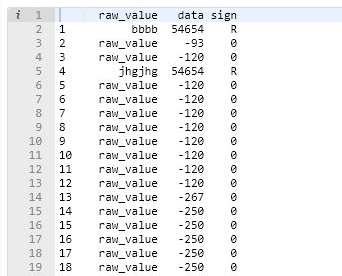
\includegraphics[width=0.85\textwidth]{figures/10/hujifd1.PNG}}
	\caption{Hasil Pengujian 1 fungsi dataset (GET)}
	\label{fig:hujifd1}
\end{figure}

\item Menampilkan data sesuai dengan field yang dimasukkan (/dataset?field=data) seperti pada gambar \ref{fig:hujifd2}.
\begin{figure}[!htbp]
	\centerline{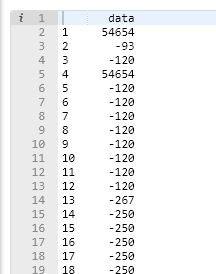
\includegraphics[width=0.85\textwidth]{figures/10/hujifd2.PNG}}
	\caption{Hasil Pengujian 2 fungsi dataset (GET)}
	\label{fig:hujifd2}
\end{figure}

\item Menampilkan data sesuai dengan field yang dimasukkan (/dataset?field=raw\_value) seperti pada gambar \ref{fig:hujifd3}.
\begin{figure}[!htbp]
	\centerline{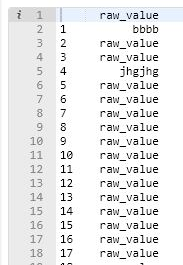
\includegraphics[width=0.85\textwidth]{figures/10/hujifd3.PNG}}
	\caption{Hasil Pengujian 3 fungsi dataset (GET)}
	\label{fig:hujifd3}
\end{figure}

\item Menampilkan data dalam bentuk Json ( /dataset?format=json) seperti pada gambar \ref{fig:hujifd4}.
\begin{figure}[!htbp]
	\centerline{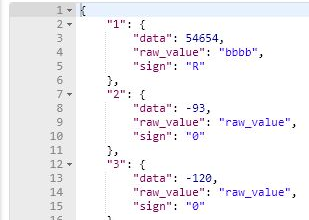
\includegraphics[width=0.85\textwidth]{figures/10/hujifd4.PNG}}
	\caption{Hasil Pengujian 4 fungsi dataset (GET)}
	\label{fig:hujifd4}
\end{figure}

\item Menampilkan 5 data teratas ( /dataset?topfive=first ) seperti pada gambar \ref{fig:hujifd5}.
\begin{figure}[!htbp]
	\centerline{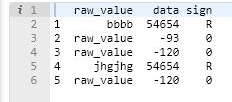
\includegraphics[width=0.85\textwidth]{figures/10/hujifd5.PNG}}
	\caption{Hasil Pengujian 5 fungsi dataset (GET)}
	\label{fig:hujifd5}
\end{figure}

\item Menampilkan data dengan urutan besar ke kecil (/dataset?field=data\&sort=descending)
seperti pada gambar \ref{fig:hujifd6}.
\begin{figure}[!htbp]
	\centerline{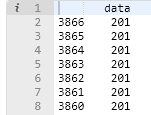
\includegraphics[width=0.85\textwidth]{figures/10/hujifd6.PNG}}
	\caption{Hasil Pengujian 6 fungsi dataset (GET)}
	\label{fig:hujifd6}
\end{figure}

\item Menampilkan 5 data teratas ( /dataset?topfive=first ) seperti pada gambar \ref{fig:hujifd7}.
\begin{figure}[!htbp]
	\centerline{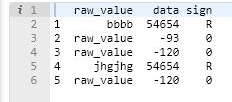
\includegraphics[width=0.85\textwidth]{figures/10/hujifd7.PNG}}
	\caption{Hasil Pengujian 7 fungsi dataset (GET)}
	\label{fig:hujifd7}
\end{figure}

\item Menampilkan data dengan urutan besar ke kecil (/dataset?field=data\&sort=descending) seperti pada gambar \ref{fig:hujifd8}.
\begin{figure}[!htbp]
	\centerline{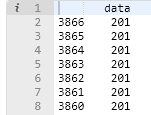
\includegraphics[width=0.85\textwidth]{figures/10/hujifd8.PNG}}
	\caption{Hasil Pengujian 8 fungsi dataset (GET)}
	\label{fig:hujifd8}
\end{figure}
\end{enumerate}

\subsection{Endpoint 2 ( URL API : /dataset/jumlah )}
Pembahasan selanjutnya yaitu tutorial untuk pembuatan endpoint kedua ( /dataset/jumlah ). Silahkan tuliskan code seperti pada listing \ref{lst:mge}:
\lstinputlisting[caption=Method Get dari Endpoint : URL API /dataset/jumlah,label={lst:mge}]{src/10/mge.py}
Pada listing \ref{lst:mge} ada fungsi jumlah, pada fungsi ini di panggil lah fungsi jumlah\_data yang bisa dieksekusi dengan beberapa nilai seperti misalnya kolom, row dan lain-lain. Bisa dilihat di bagian alur manipulasi data. 
Tutorial :
\begin{enumerate}
\item Silahkan melanjutkan contoh file diatas
\item Masukkan endpoint dataset/jumlah
\item Terapkan method Get : dengan fungsi jumlah dimana di dalamnya terdapat argument untuk parameter from ( row dan column )
\item Penjelasan Parameter From :
\begin{itemize}
\item Column		:Akan mengambil dan menampilkan jumlah kolom sesuai dengan kolom yang ada pada file CSV yang dieksekusi.
\item Row		:Akan mengambil dan menampilkan jumlah baris sesuai dengan baris yang ada pada file CSV yang dieksekusi.
\end{itemize}
\item Kemudian pada argument/parameter from tersebut, fungsi jumlah\_data dijadikan sebagai respon
\item Fungsi jumlah\_data akan menghitung berapa banyak jumlah baris dan kolom pada data ( tertentu, sesuai dengan parameternya yang di get)
\item Kemudian apabila pengeksekusian tanpa dibarengi dengan argument/parameter maka akan menampilkan jumlah keseluruhan.
\end{enumerate}

\begin{itemize}
\item HASIL PENGUJIAN ( Fungsi Dataset/jumlah , method: GET ):
\end{itemize}
\begin{enumerate}
\item Menampilkan jumlah data secara keseluruhan ( /dataset/jumlah ) seperti pada gambar \ref{fig:hujifdj1}.
\begin{figure}[!htbp]
	\centerline{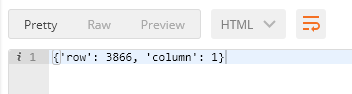
\includegraphics[width=0.85\textwidth]{figures/10/hujifdj1.PNG}}
	\caption{Hasil Pengujian 1 fungsi dataset/jumlah (GET)}
	\label{fig:hujifdj1}
\end{figure}

\item Menampilkan jumlah data row (/dataset/jumlah?from=row) seperti pada gambar \ref{fig:hujifdj2}.
\begin{figure}[!htbp]
	\centerline{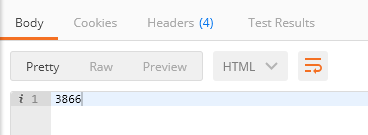
\includegraphics[width=0.85\textwidth]{figures/10/hujifdj2.PNG}}
	\caption{Hasil Pengujian 2 fungsi dataset/jumlah (GET)}
	\label{fig:hujifdj2}
\end{figure}

\item  Menampilkan jumlah data row (/dataset/jumlah?from=column) seperti pada gambar \ref{fig:hujifdj3}.
\begin{figure}[!htbp]
	\centerline{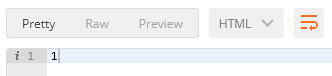
\includegraphics[width=0.85\textwidth]{figures/10/hujifdj3.PNG}}
	\caption{Hasil Pengujian 3 fungsi dataset/jumlah (GET)}
	\label{fig:hujifdj3}
\end{figure}
\end{enumerate}

\subsection{Endpoint 3 ( URL API : /dataset/<id> )}
Pembahasan selanjutnya yaitu tutorial untuk pembuatan endpoint ketiga ( /dataset/<id> ). Silahkan perhatikan dan ikuti file seperti pada listing \ref{lst:mege}:
\lstinputlisting[caption=Method Get dari Endpoint : URL API /dataset/<id>,label={lst:mege}]{src/10/mege.py}
Pada listing \ref{lst:mege} terdapat fungsi detail. Di dalam fungsi tersebut dipergunakan untuk pengeksekusian data memakai fungsi yang diperlukan penentuan index id. Jadi kebanyakan dari hasil fungsi yang dipanggil dan dihubungkan kedalam fungsi detail. 
Tutorial :
\begin{enumerate}
\item Silahkan melanjutkan contoh file diatas
\item Masukkan endpoint dataset/id
\item Terapkan method Get : dengan fungsi jumlah dimana di dalamnya terdapat argument untuk parameter field ( raw\_value, data, sign ) dan format ( json )
\item Penjelasan Parameter :
\begin{itemize}
\item All	:Menampilkan data sesuai index id yang dipanggil tanpa parameter tertentu.
\item Field	:Menampilkan dan mengambil data dari kolom tertentu dan disesuaikan dengan index id yang telah dipanggil
\item Format	:Menampilkan dan mengambil data dengan format tulisan JSON dan RAW sesuai dengan index id yang dipanggil.
\end{itemize}
\item Kemudian pada argument/parameter field tersebut, fungsi get\_row\_field dijadikan sebagai respon
\item Fungsi get\_row\_field akan mengambil data dari row tersebut sesuai dengan field yang dimasukkan 
\item Selanjutnya pada argument/parameter format, fungsi jsonify(get\_all\_data\_json) dijadikan sebagai respon
\item Fungsi get\_all\_data\_json akan mengambil data dari id tersebut dan ditampilkan dengan format json string. 
 \item Kemudian reload\_data akan menampilkan data terbaru setelah dilakukan perintah delete.
 \item Setelah semuanya selesai, maka tutorial untuk tahapan ini juga sudah berhasil.
\end{enumerate}
\begin{itemize}
\item HASIL PENGUJIAN ( Fungsi Dataset/<id>, method: GET ):
\end{itemize}
\begin{enumerate}
\item Menampilkan data berdasarkan id ( /dataset/<id>) seperti pada gambar \ref{fig:hujifdi1}.
\begin{figure}[!htbp]
	\centerline{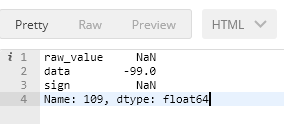
\includegraphics[width=0.85\textwidth]{figures/10/hujifdi1.PNG}}
	\caption{Hasil Pengujian 1 fungsi dataset/<id> (GET)}
	\label{fig:hujifdi1}
\end{figure}

\item Menampilkan data sesuai id dengan format json (/dataset/1?format=json) seperti pada gambar \ref{fig:hujifdi2}.
\begin{figure}[!htbp]
	\centerline{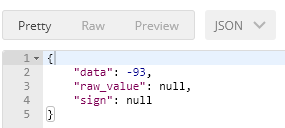
\includegraphics[width=0.85\textwidth]{figures/10/hujifdi2.PNG}}
	\caption{Hasil Pengujian 2 fungsi dataset/<id> (GET)}
	\label{fig:hujifdi2}
\end{figure}

\item Menampilkan data sesuai id dengan format raw (/dataset?format=raw) seperti pada gambar \ref{fig:hujifdi3}.
\begin{figure}[!htbp]
	\centerline{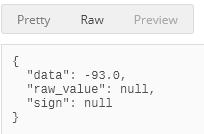
\includegraphics[width=0.85\textwidth]{figures/10/hujifdi3.PNG}}
	\caption{Hasil Pengujian 3 fungsi dataset/<id> (GET)}
	\label{fig:hujifdi3}
\end{figure}

Gambar 9.14. Hasil pengujian 3 fungsi dataset/<id> (GET)
\end{enumerate}

\subsection{Endpoint 4 ( URL API : /info )}
Pembahasan selanjutnya ialah untuk endpoint terakhir yaitu endpoint info. Silahkan perhatikan file dibawah kemudian silahkan anda ikuti seperti pada listing \ref{lst:mgei}:
\lstinputlisting[caption=Method Get dari Endpoint : URL API /dataset/info,label={lst:mgei}]{src/10/mgei.py}

Pada file ini cukup sederhana fungsinya yaitu hanya untuk mendapatkan data berupa deskripsi bawaan dari library ( bentuknya akan berbeda dari GET data sebelumnya )

Tutorial :
\begin{enumerate}
\item Silahkan melanjutkan contoh file diatas
\item Masukkan endpoint info
\item Terapkan method Get : dengan fungsi info diatas
\item Setelah itu silahkan eksekusi menggunakan CMD maka hasilnya akan sebagai berikut :
\end{enumerate}
\begin{itemize}
\item HASIL PENGUJIAN ( Fungsi info, method: GET ):
\end{itemize}
Menampilkan data berdasarkan info yang disimpan library pandas ( /info) seperti pada gambar \ref{fig:hujiinf}.
\begin{figure}[!htbp]
	\centerline{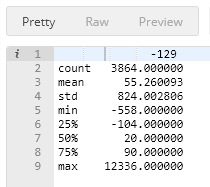
\includegraphics[width=0.85\textwidth]{figures/10/hujiinf.PNG}}
	\caption{Hasil Pengujian 1 fungsi dataset/info (GET)}
	\label{fig:hujiinf}
\end{figure}

\section {Mendapatkan Parameter GET Python Flask}
\subsection{Penjelasan Parameter GET Python Flask}
Parameter GET pada Python Flask ini saya lampirkan dan ujikan dalam bentuk file penuh dengan beberapa fungsi. File tersebut bernama Main.py. Untuk penerapan lebih dan contoh GETnya sudah saya tampilkan dan jelaskan sebelumnya pada point contoh URL GET. 
Namun, penggabungannya bersama Flask Python ada pada file ini. Silahkan diperhatikan penjelasan dan tutorialnya dan semoga dapat dimengerti. 

Namun sebelum melanjutkan tutorial silahkan pertama-tama kita harus memastikan beberapa hal yaitu :
\begin{enumerate}
\item Persiapan Python : Instalasi Python 3.6
Instalasi Python dapat ditemukan di penjelasan sebelumnya ( Sub Menu 1 ). Namun apabila masih belum paham dapat mengikuti langkah-langkah berikut:
\begin{itemize}
\item Pertama-tama silahkan download software dari python versi 3 di laptop anda.
\item Download python versi 3.6.3 dari situs web resminya yaitu https://www.python.org/
\item Silahkan sesuaikan dengan kapasitas laptop anda, bisa yang win 32 atau yang win 64 ( 32 bit / 64 bit )
\item Contoh downloadnya seperti pada gambar \ref{fig:inspy}.
\begin{figure}[!htbp]
	\centerline{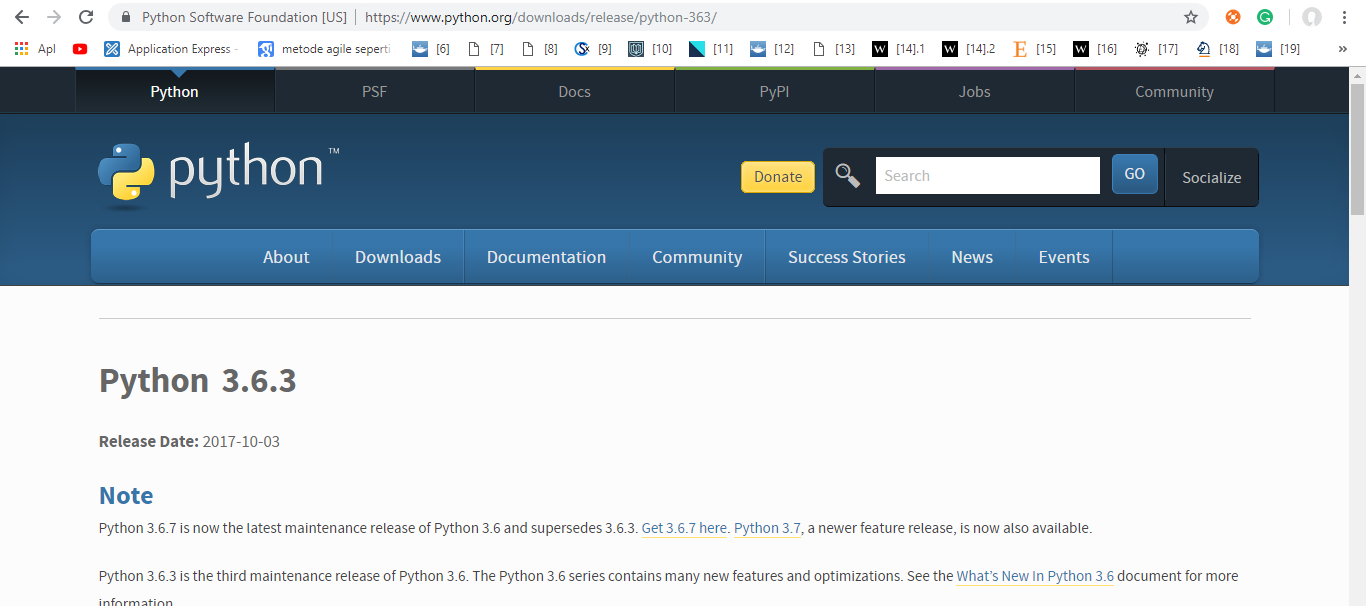
\includegraphics[width=0.85\textwidth]{figures/10/inspy.PNG}}
	\caption{Instalasi Python}
	\label{fig:inspy}
\end{figure}

\item Setelah berhasil melakukan pengunduhan/download aplikasi python tersebut, maka silahkan lakukan instalasi
\item Instalasi dapat dilakukan seperti instalasi biasa pada umumnya
\item Setelah selesai instalasi python, silahkan check di Command Prompt, apakah Pythonnya telah terbaca / running disesuaikan dengan laptop anda atau belum.
\item Contoh pengecekan di Command Prompt seperti pada gambar \ref{fig:pyc}.
\begin{figure}[!htbp]
	\centerline{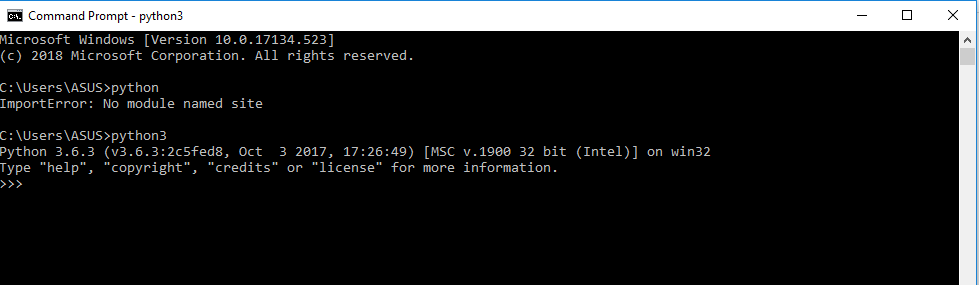
\includegraphics[width=0.85\textwidth]{figures/10/pyc.PNG}}
	\caption{Python CMD}
	\label{fig:pyc}
\end{figure}

\item Apabila tampilannya telah sesuai dengan contoh diatas, maka python anda siap digunakan. 
\item Pastikan python yang terbaca versi 3.6.3 atau bahkan belum ada sama sekali silahkan lakukan konfigurasi ini :
\begin{itemize}
\item Silahkan buka Control Panel anda
\item Pilih System and Security
\item Kemudian pilih lagi system
\item Lalu di bagian kiri tampilan ada sub menu Advanced system setting
\item Pada sub menu tersebut silahkan pilih button Environment Variabel
\item Silahkan ganti path dengan C:/Python36 dan C:/Python36/Scripts ( Lokasi anda menyimpan mentahan python yang telah anda install tadi )
\item Maka tampilannya akan seperti pada gambar \ref{fig:dme}.
\begin{figure}[!htbp]
	\centerline{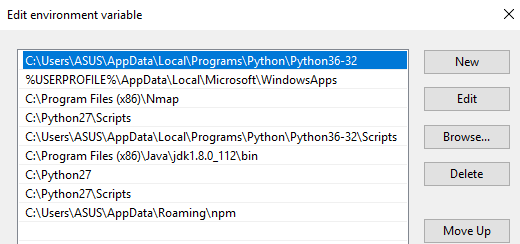
\includegraphics[width=0.85\textwidth]{figures/10/dme.PNG}}
	\caption{Device Manager ( Env )}
	\label{fig:dme}
\end{figure}

\item Jangan lupa untuk memasukkan script dari python sehingga benar-benar bisa terbaca untuk pipnya.
\item Silahkan klik button ok sampai selesai
\item Setelah itu, lakukan pengecekan ulang di Command Prompt maka hasilnya akan berubah menjadi versi 3.6.3 
\item Setelah semua tahap di atas selesai, maka silahkan lanjutkan ke tahap berikutnya
\end{itemize}
\end{itemize}

\item Persiapan Flask

Tutorial selanjutnya ialah kita akan menginstall Framework Flask di komputer/laptop kita sehingga bisa digunakan untuk tutorial selanjutnya. Untuk teman-teman ketahui flask sendiri merupakan microframework dari python, dengan penggunaannya, aktivas apapun yang kita lakukan baik pengolahan data dll akan terasa lebih mudah dan rapih, kurang lebih seperti itu.

Instalasi Flask dapat ditemukan di penjelasan sebelumnya ( Sub Menu 7 ). Namun apabila masih belum paham dapat mengikuti langkah-langkah berikut :
\begin{itemize}
\item Pertama-tama silahkan nyalakan laptop / komputer anda
\item Kemudian apabila komputer / laptop anda telah bisa digunakan silahkan buka web browser 
\item Web browser yang digunakan bisa Chrome. Mozilla Firefox dll sesuai dengan keinginan anda.
\item Selanjutnya pada web browser silahkan kunjungi website resmi berikut : https://pypi.org/project/Flask/
\item Pada website tersebut silahkan download Flask
\item Contohnya nampak seperti pada gambar \ref{fig:insfla}.
\begin{figure}[!htbp]
	\centerline{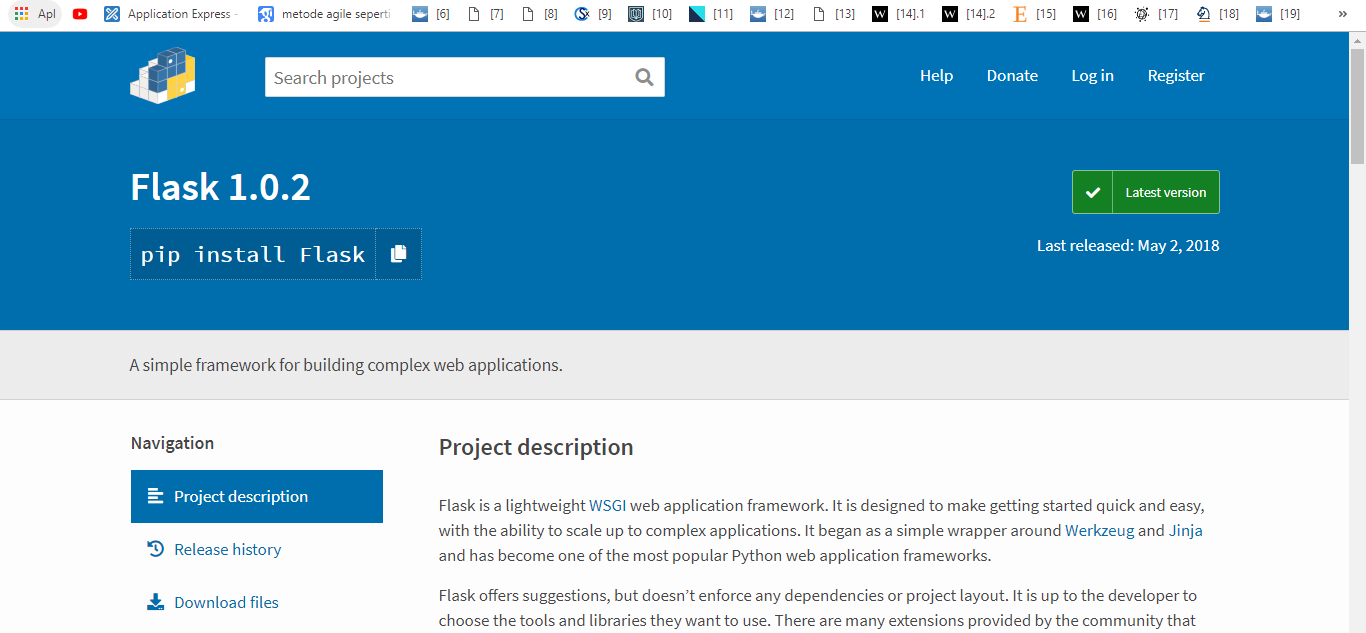
\includegraphics[width=0.85\textwidth]{figures/10/insfla.PNG}}
	\caption{Instalasi Flask}
	\label{fig:insfla}
\end{figure}

\item Setelah di download silahkan buka Command Prompt di komputer/laptop anda
\item Kemudian silahkan ketikkan perintah ( pip install flask )
\item Setelah mengetikkan perintah tersebut, silahkan tekan enter maka prosesnya akan belajar
\item Silahkan tunggu hasilnya
\item Hasilnya akan nampak seperti pada gambar \ref{fig:ifc}.
\begin{figure}[!htbp]
	\centerline{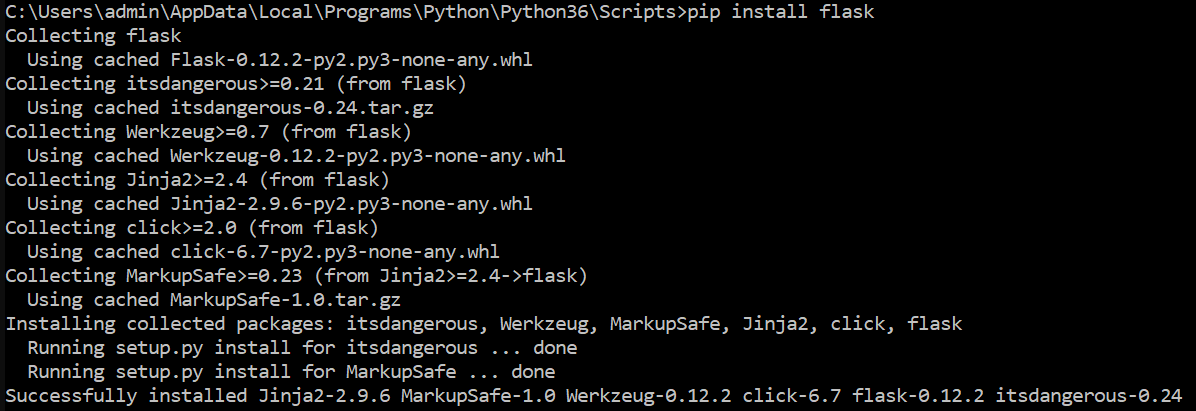
\includegraphics[width=0.85\textwidth]{figures/10/ifc.PNG}}
	\caption{Install Flask di CMD}
	\label{fig:ifc}
\end{figure}

\item Apabila tampilan pada proses di komputer/laptop anda telah nampak seperti gambar yang dicontohkan maka prosesnya berhasil
\item Dan apabila masih terjadi error maka silahkan lakukan kembali langkah-langkahnya, bisa saja anda melewatkan beberapa point pada tutorial ini
\item Setelah flasknya terpasang di komputer/laptop anda maka silahkan lanjutkan ke tutorial selanjutnya.
\end{itemize}

\item Persiapan Library Pandas ( untuk menyesuaikan dengan file CSV yang dieksekusi.

Tutorial selanjutnya ialah kita akan menginstall Library Pandas di komputer/laptop kita sehingga bisa digunakan untuk tutorial selanjutnya. Untuk teman-teman ketahui pandas sendiri merupakan library dari bahasa pemrograman Python. Library ini digunakan untuk pemrosesan data analitik. Mengapa kita gunakan? Karena memang pandas ini akan mengolah data analitik dari CSV file yang berisikan data sinyal gelombang otak yang kita baca dan tangkap dari aktifitas tertentu ( lampu sein saat bermotor ). Nah mari kita mulai:

Instalasi Pandas dapat ditemukan di penjelasan sebelumnya ( Sub Menu 7 ). Namun apabila masih belum paham dapat mengikuti langkah-langkah berikut :
\begin{itemize}
\item Pertama-tama silahkan nyalakan laptop / komputer anda
\item Kemudian apabila komputer / laptop anda telah bisa digunakan silahkan buka web browser 
\item Web browser yang digunakan bisa Chrome. Mozilla Firefox dll sesuai dengan keinginan anda.
\item Selanjutnya pada web browser silahkan kunjungi website resmi berikut : https://pypi.org/project/pandas/
\item Pada website tersebut silahkan download Pandas
\item Contohnya nampak seperti pada gambar \ref{fig:inspa}.
\begin{figure}[!htbp]
	\centerline{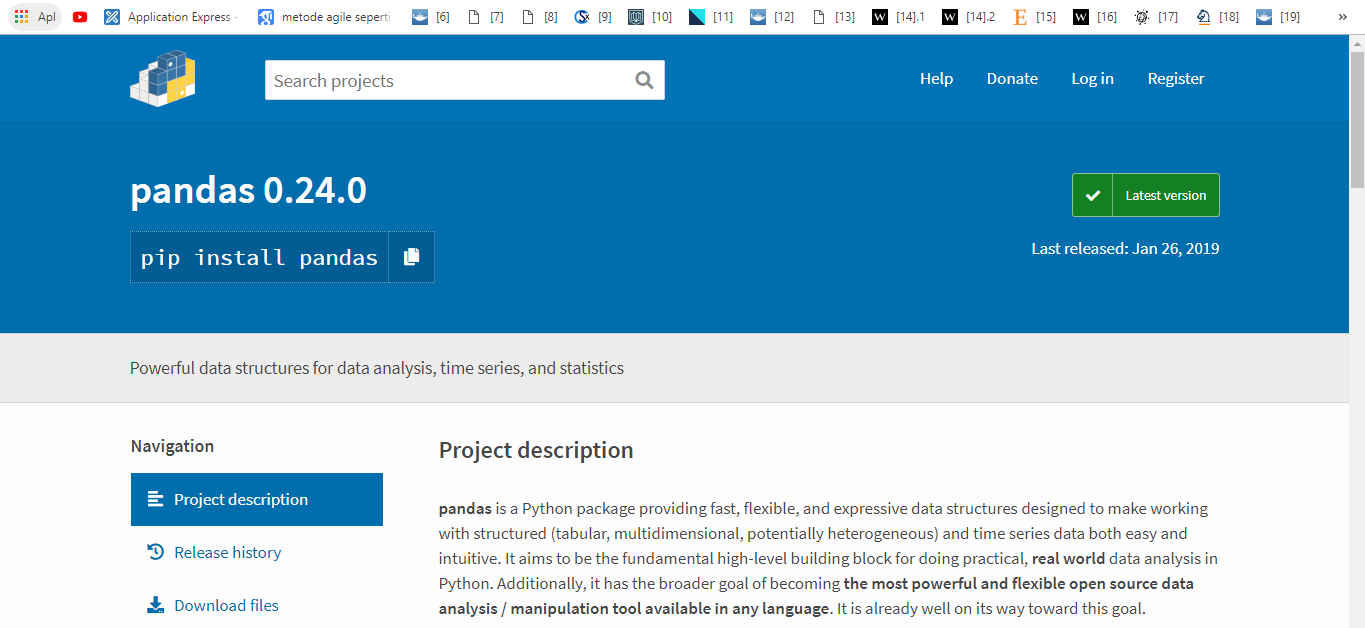
\includegraphics[width=0.85\textwidth]{figures/10/inspa.PNG}}
	\caption{Instalasi Pandas}
	\label{fig:inspa}
\end{figure}

\item Setelah di download silahkan buka Command Prompt di komputer/laptop anda
\item Kemudian silahkan ketikkan perintah ( pip install pandas )
\item Setelah mengetikkan perintah tersebut, silahkan tekan enter maka prosesnya akan belajar
\item Silahkan tunggu hasilnya
\item Hasilnya akan nampak seperti pada gambar \ref{fig:ipc}.
\begin{figure}[!htbp]
	\centerline{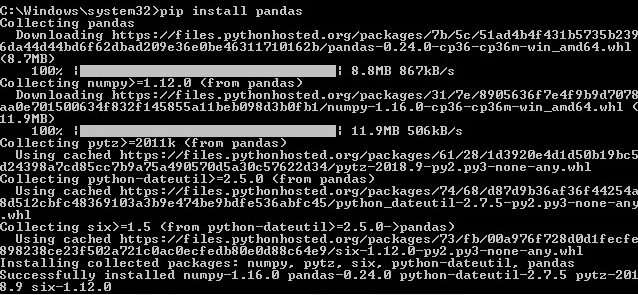
\includegraphics[width=0.85\textwidth]{figures/10/ipc.PNG}}
	\caption{Install Pandas di CMD}
	\label{fig:ipc}
\end{figure}

\item Apabila tampilan pada proses di komputer/laptop anda telah nampak seperti gambar yang dicontohkan maka prosesnya berhasil
\item Dan apabila masih terjadi error maka silahkan lakukan kembali langkah-langkahnya, mungkin anda melewatkan beberapa point pada tutorial ini
\item Setelah pandasnya terpasang di komputer/laptop anda maka silahkan lanjutkan ke tutorial selanjutnya
\end{itemize}
\end{enumerate}

Filenya yang akan dijadikan tutorial yaitu seperti pada listing \ref{lst:mpf}:
\lstinputlisting[caption=File Main.py Python Flask,label={lst:mpf}]{src/10/mpf.py}

Penjelasan Lengkap :
\begin{enumerate}
\item Penjelasan I : Main.py
\lstinputlisting[caption=Penjelasan I : Main.py,label={lst:pm1}]{src/10/pm1.py}

Listing \ref{lst:pm1} merupakan codingan untuk mendefinisikan framework flask, beberapa module yang digunakan untuk mengeksekusi fungsi seperti request, jsonify dan juga ada library pandas yang digunakan untuk pengeksekusian data analitik seperti file csv yang digunakan. Pada code juga dilakukan pemanggilan file-file yang di dalamnya telah terdapat masing-masing fungsi yang telah dijelaskan sebelumnya sehingga semuanya dapat dieksekusi dalam 1 framework Flask Python.
Langkah-langkah :
\begin{itemize}
\item Silahkan buka sublime anda
\item Kemudian buatlah file baru dengan nama Main.py
\item Kemudian silahkan masukkan perintah import
\item Perintah import apa saja? Silahkan mengimportkan perintah/file sesuai dengan contoh pada gambar
\end{itemize}

\item Penjelasan II : Main.py
\lstinputlisting[caption=Penjelasan II : Main.py,label={lst:pm2}]{src/10/pm2.py}

Listing \ref{lst:pm2}  dijelaskan bahwa file yang dieksekusi ialah Book1.csv kemudian variabel dataframenya akan memanggil fungsi load\_data yang di dalamnya juga didefinisikan variabel filename. Indexnya sendiri ialah 1. Untuk fungsi reload\_data memiliki variabel fname dan dfname .
\begin{itemize}
\item Silahkan lanjutkan pada file main.py
\item Kemudian masukkan perintah diatas
\item Variabel Filename disesuaikan dengan file yang akan diolah ( misal Book1.csv)
\item Kemudian jangan lupa masukkan variabel dataframe ( tentunya untuk pengolahan data secara keseluruhan )
\item Lalu, difungsikan juga reload\_data ( mengupdate data ketika ada perubahan )
\item Jangan lupa untuk menambahkan dataframe.to\_csv sehingga parameternya akan dipisahkan oleh perintah ( sep = “ : ” ) dengan index=false
\item Selanjutnya silahkan return variabel dataframe
\end{itemize}

\item Penjelasan III : Main.py
Penjelasan ini terdiri dari penjelasan untuk setiap endpoint dari Method GETnya.
\begin{itemize}
\item Endpoint 1 ( URL API : /dataset ): Telah dijelaskan pada point contoh URL Get. Halaman 7-14
\item Endpoint 2 ( URL API : /dataset/jumlah ): Telah dijelaskan pada point contoh URL Get. Halaman 7-14
\item Endpoint 3 ( URL API : /dataset/<id> ): Telah dijelaskan pada point contoh URL Get. Halaman 7-14
\item Endpoint 4 ( URL API : /info ): Telah dijelaskan pada point contoh URL Get. Halaman 7-14
\end{itemize}

\item Penjelasan IV : Main.py
\lstinputlisting[caption=Penjelasan IV : Main.py,label={lst:pm4}]{src/10/pm4.py}

Listing \ref{lst:pm4} difungsikan untuk mengeksekusi inputan yang telah dimasukkan kedalam flask yang menjadi body dari code tersebut yaitu Main.py . Kemudian ketika dijalankan hasilnya true maka aplikasinya akan jalan sesuai dengan yang seharusnya
\end{enumerate}

\section{Penanganan Error}
\subsection{Error 1}
\begin{enumerate}
\item Silahkan jalankan kembali CMD anda
\item Kemudian masuk ke Directory tempat anda menyimpan file main.py
\item Kemudian masukkan perintah berikut :
\verb|Env/scripts/activate|
\item Maksud dari Code tersebut ialah untuk mengaktifkan scriptnya python3
\item Maka hasilnya akan nampak seperti pada gambar \ref{fig:am2}.
\begin{figure}[!htbp]
	\centerline{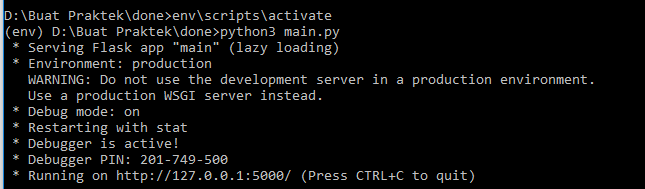
\includegraphics[width=0.85\textwidth]{figures/10/am2.PNG}}
	\caption{Aktivasi main.py 2 pada contoh kasus 3}
	\label{fig:am2}
\end{figure}

\item Apabila hasilnya seperti gambar diatas maka filenya telah berjalan dengan baik
\item Bisa dilihat, untuk URL APInya sudah muncul jadi silahkan copy dan buktikan menggunakan POSTMAN atau browser biasa.
\item Hasilnya seperti berikut, apabila dieksekusi sesuai endpoint.
\item Misalnya endpoint : dataset/<id>  seperti pada gambar \ref{fig:huji1}.
\begin{figure}[!htbp]
	\centerline{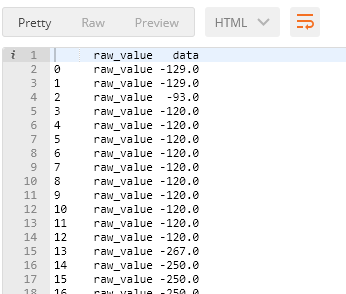
\includegraphics[width=0.85\textwidth]{figures/10/huji1.PNG}}
	\caption{Hasil pengujian 1 untuk error 9 pada contoh kasus 3}
	\label{fig:huji1}
\end{figure}

\item Kemudian apabila muncul ERROR seperti pada gambar \ref{fig:err1}.
\begin{figure}[!htbp]
	\centerline{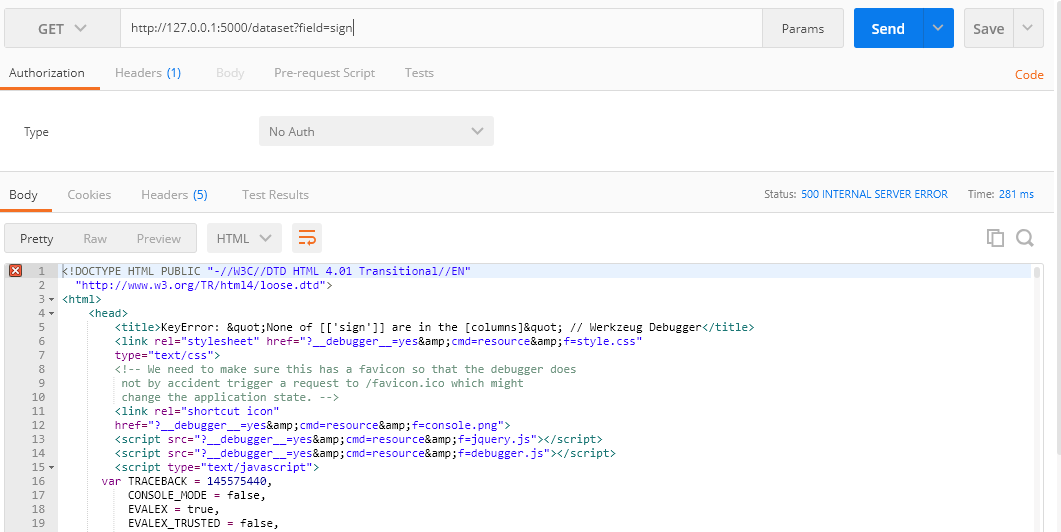
\includegraphics[width=0.85\textwidth]{figures/10/err1.PNG}}
	\caption{Error 1 untuk error 9 pada contoh kasus 3}
	\label{fig:err1}
\end{figure}

\item Maka tindakannya seperti berikut:
\begin{itemize}
\item Perhatikan terlebih dahulu request yang diminta
\item Request yang diminta yaitu field dengan parameter kolom sign
\item Silahkan diperiksa dulu apakah pada file yang ingin di get, kolom tersebut masih ada.
\item Apabila tidak ada, maka silahkan masukkan file baru yang ada kolom signnya
\item Kemudian silahkan jalankan kembali requestnya
\item Maka hasilnya akan nampak seperti pada gambar \ref{fig:huji2}.
\begin{figure}[!htbp]
	\centerline{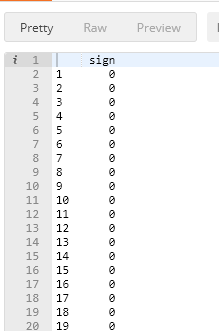
\includegraphics[width=0.85\textwidth]{figures/10/huji2.PNG}}
	\caption{Hasil pengujian 2 untuk error 9 pada contoh kasus 3}
	\label{fig:huji2}
\end{figure}
\end{itemize}
\end{enumerate}

\subsection{Error 2}
\begin{enumerate}
\item Silahkan jalankan kembali CMD anda
\item Kemudian masuk ke Directory tempat anda menyimpan file main.py
\item Kemudian masukkan perintah berikut : \verb|Env/scripts/activate|
\item Maksud dari Code tersebut ialah untuk mengaktifkan scriptnya python3
\item Maka hasilnya akan nampak seperti pada gambar \ref{fig:am3}.
\begin{figure}[!htbp]
	\centerline{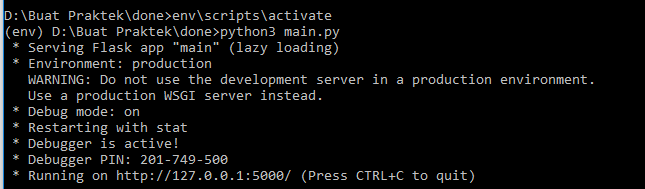
\includegraphics[width=0.85\textwidth]{figures/10/am3.PNG}}
	\caption{Aktivasi main.py 3 pada contoh kasus 3}
	\label{fig:am3}
\end{figure}

\item Apabila hasilnya seperti gambar diatas maka filenya telah berjalan dengan baik
\item Bisa dilihat, untuk URL APInya sudah muncul. Silahkan copy dan buktikan menggunakan POSTMAN atau browser biasa.
\item Hasilnya seperti berikut, apabila dieksekusi sesuai endpoint.
\item Misalnya endpoint : dataset seperti pada gambar \ref{fig:hu1}.
\begin{figure}[!htbp]
	\centerline{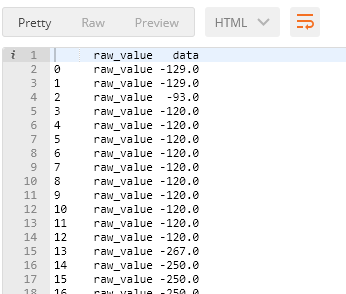
\includegraphics[width=0.85\textwidth]{figures/10/hu1.PNG}}
	\caption{Hasil pengujian 1 untuk error 10 pada contoh kasus 3}
	\label{fig:hu1}
\end{figure}

\item Kemudian apabila muncul ERROR seperti pada gambar \ref{fig:er1}.
\begin{figure}[!htbp]
	\centerline{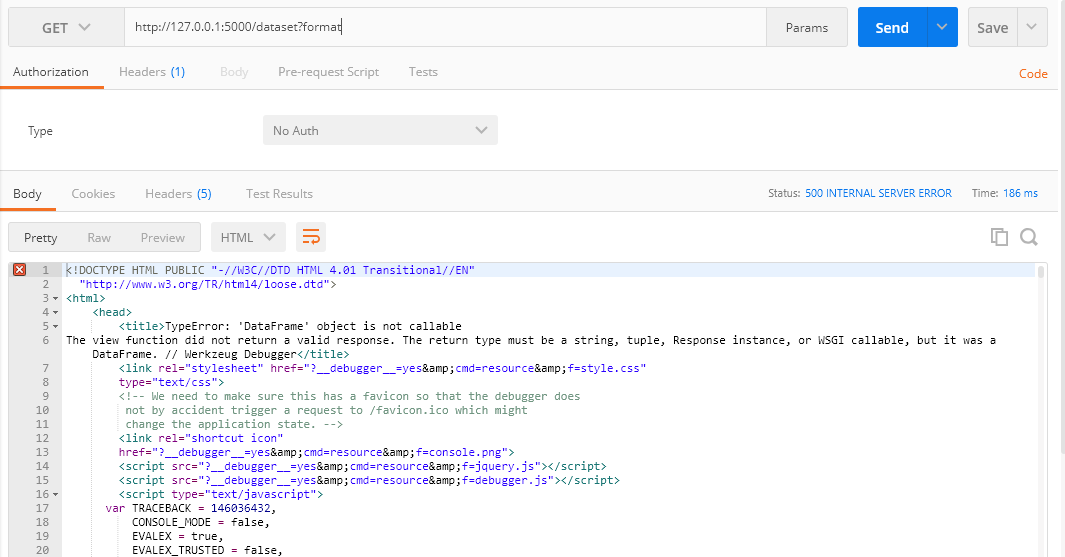
\includegraphics[width=0.85\textwidth]{figures/10/er1.PNG}}
	\caption{Error 1 untuk error 10 pada contoh kasus 3}
	\label{fig:er1}
\end{figure}

\item Maka tindakannya seperti berikut	:
\begin{itemize}
\item Perhatikan terlebih dahulu request yang diminta
\item Request yang diminta yaitu format
\item Silahkan diperiksa kembali apakah pada codingan API nya terdapat request global untuk parameter Format
\item Ada, namun harus disertai dengan parameter yang lain
\item Seperti ini : ?format=json
\item Ketika requestnya seperti itu, maka hasilnya akan muncul
\item Silahkan jalankan kembali requestnya
\item Maka hasilnya akan nampak seperti pada gambar \ref{fig:hu2}.
\begin{figure}[!htbp]
	\centerline{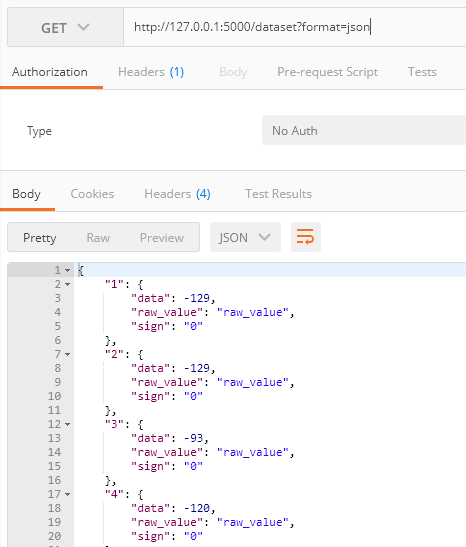
\includegraphics[width=0.85\textwidth]{figures/10/hu2.PNG}}
	\caption{Hasil pengujian 2 untuk error 10 pada contoh kasus 3}
	\label{fig:hu2}
\end{figure}
\end{itemize}
\end{enumerate}

\subsection{Error 3}
\begin{enumerate}
\item Silahkan jalankan kembali CMD anda
\item Kemudian masuk ke Directory tempat anda menyimpan file main.py
\item Kemudian masukkan perintah berikut : Env/scripts/activate
\item Maksud dari Code tersebut ialah untuk mengaktifkan scriptnya python3
\item Maka hasilnya akan nampak seperti pada gambar \ref{fig:am4}.
\begin{figure}[!htbp]
	\centerline{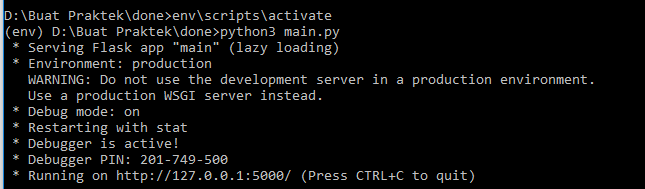
\includegraphics[width=0.85\textwidth]{figures/10/am4.PNG}}
	\caption{Aktivasi main.py 4 pada contoh kasus 3}
	\label{fig:am4}
\end{figure}

\item Apabila hasilnya seperti gambar diatas maka filenya telah berjalan dengan baik
\item Bisa dilihat, untuk URL APInya sudah muncul jadi silahkan copy dan buktikan menggunakan POSTMAN atau browser biasa.
\item Hasilnya seperti berikut, apabila dieksekusi sesuai endpoint.
 \item Misalnya endpoint : dataset/<id> seperti pada gambar \ref{fig:hu11}.
\begin{figure}[!htbp]
	\centerline{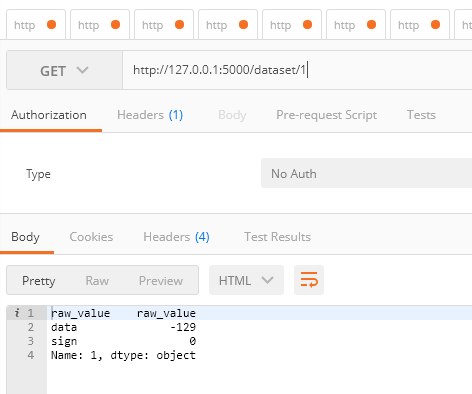
\includegraphics[width=0.85\textwidth]{figures/10/hu11.PNG}}
	\caption{Hasil pengujian 1 untuk error 11 pada contoh kasus 3}
	\label{fig:hu11}
\end{figure}

\item Kemudian apabila muncul ERROR seperti pada gambar \ref{fig:err11}.
\begin{figure}[!htbp]
	\centerline{\includegraphics[width=0.85\textwidth]{figures/10/err11.PNG}}
	\caption{Error 1 untuk error 11 pada contoh kasus 3}
	\label{fig:err11}
\end{figure}

\item Maka tindakannya seperti berikut :
\begin{itemize}
\item Perhatikan terlebih dahulu request yang diminta
\item Request yang diminta yaitu id 4000
\item Silahkan diperiksa kembali apakah pada filenya ada id 4000 yang bisa diubah
\item Tidak ada, maka dari itu silahkan coba  diganti dengan id yang terdapat dala file tersebut
\item Seperti ini : dataset/2000
\item Ketika requestnya seperti itu maka hasilnya akan muncul
\item Silahkan jalankan kembali requestnya
\item Maka hasilnya akan nampak seperti pada gambar \ref{fig:hu21}.
\begin{figure}[!htbp]
	\centerline{\includegraphics[width=0.85\textwidth]{figures/10/hu21.PNG}}
	\caption{Hasil pengujian 2 untuk error 11 pada contoh kasus 3}
	\label{fig:hu21}
\end{figure}
\end{itemize}

\item Maka id yang ke POST atau Update yaitu id 2000 dengan isi yang dapat diliat seperti pada gambar diatas.
\end{enumerate}


\bibliographystyle{IEEEtran}
%\def\bibfont{\normalsize}
\bibliography{references}


%%%%%%%%%%%%%%%
%%  The default LaTeX Index
%%  Don't need to add any commands before \begin{document}
\printindex

%%%% Making an index
%%
%% 1. Make index entries, don't leave any spaces so that they
%% will be sorted correctly.
%%
%% \index{term}
%% \index{term!subterm}
%% \index{term!subterm!subsubterm}
%%
%% 2. Run LaTeX several times to produce <filename>.idx
%%
%% 3. On command line, type  makeindx <filename> which
%% will produce <filename>.ind
%%
%% 4. Type \printindex to make the index appear in your book.
%%
%% 5. If you would like to edit <filename>.ind
%% you may do so. See docs.pdf for more information.
%%
%%%%%%%%%%%%%%%%%%%%%%%%%%%%%%

%%%%%%%%%%%%%% Making Multiple Indices %%%%%%%%%%%%%%%%
%% 1.
%% \usepackage{multind}
%% \makeindex{book}
%% \makeindex{authors}
%% \begin{document}
%%
%% 2.
%% % add index terms to your book, ie,
%% \index{book}{A term to go to the topic index}
%% \index{authors}{Put this author in the author index}
%%
%% \index{book}{Cows}
%% \index{book}{Cows!Jersey}
%% \index{book}{Cows!Jersey!Brown}
%%
%% \index{author}{Douglas Adams}
%% \index{author}{Boethius}
%% \index{author}{Mark Twain}
%%
%% 3. On command line type
%% makeindex topic
%% makeindex authors
%%
%% 4.
%% this is a Wiley command to make the indices print:
%% \multiprintindex{book}{Topic index}
%% \multiprintindex{authors}{Author index}

\end{document}

